\documentclass[10pt]{mcmthesis}
\mcmsetup{%CTeX = false,                       %% ʹÓà CTeX Ì×װʱ£¬ÉèÖÃΪ true
        tcn = 2312787, problem = D,             %% tcn is team control number
        sheet = true, titleinsheet = true,    %% sheet stands for summary sheet
        titlepage = false, abstract = true}    %% titlepage represents abstract page, true or false

%\usepackage{palatino}   %%COMAP¹Ù·½°æÎï×ÖÌå
%\usepackage{times}      %%ÂÞÂí×ÖÌ壬ֻ¶ÔÕýÎÄÆð×÷ÓÃ
\usepackage{txfonts}     %%Êýѧ¹«Ê½ÂÞÂí×ÖÌ壬¶Ô¹«Ê½ºÍÕýÎĶ¼Æð×÷ÓÃ
\usepackage {subcaption}
\usepackage{geometry}
\usepackage{float}
\geometry{a4paper,left=2.3cm,right=2.3cm,top=2.5cm,bottom=2cm}
% \geometry{a4paper,scale=0.9}
\usepackage{indentfirst}
\setlength{\parindent}{2em}
\usepackage{setspace}


\newcommand{\subsubsubsection}[1]{\paragraph{#1}\mbox{}\\}
\setcounter{secnumdepth}{4} % how many sectioning levels to assign numbers to
\setcounter{tocdepth}{2} % how many sectioning levels to show in ToC


\title{\textbf{ Modeling and Optimization of the Priority Sequencing for SDGs Based on Multi-objective Optimization}}
\author{\team}
\date{\today}
\begin{document}

\begin{summary}
Currently, the United Nations is preparing to implement 17 Sustainable Development Goals (SDGs), and considering that these SDGs have important interactions with each other, it is a challenging task to determine their priorities to allow for greater improvements in the lives of many people around the world. In order to better handle this challenge, this paper investigates the modelling and optimization methods of this problem from a multi-objective optimization perspective, so that it can provide effective support to the United Nations or other organizations in making such decisions.

Firstly, a network structure is constructed to reflect the weight of the influence relationship between different SDGs, and the influence matrix of different priorities on the implementation time of SDGs is also constructed based on this influence relationship.

Secondly, based on the influence relationship between the priorities of SDGs on the investment cost and implementation time, a multi-objective optimization model of the problem is established with the priority sequence of different SDGs as the decision variables and the minimization of the overall investment cost and total completion time of all SDGs as the optimization objectives. In the modelling process, the novelty of this paper is that we construct mathematical models for three different cases based on the actual situation of whether different SDGs can be carried out simultaneously: (1) SDGs cannot overlap with each other (i.e., only one SDG can be invested at a time), (2) two adjacent SDGs can overlap with each other, and (3) multiple SDGs can overlap with each other. It should be noted that in the models the execution time and investment money of each SDG varies with the priority sequence. That is, the values of the current SDG are affected by the SDGs that are positioned before the current SDG in the priority sequence.

Thirdly, for each of these three different cases, a decomposition-based multi-objective evolutionary algorithm is proposed to solve the corresponding model. 

Fourthly, based on the in-depth analysis of the experimental results of the three models, the corresponding conclusions are drawn, which are our answers to the requirements of the contest.

Finally, based on the characteristics of the constructed models and algorithms, their value of the generalized application to other organizations or enterprises in making investments or project construction is discussed.


\noindent
\textbf{Key Words:}
Multi-objective optimization, priority sequence-dependent investment and execution time, evolutionary algorithm

\end{summary}


\maketitle



%\newpage
%\thispagestyle{empty}
%\begin{center}
%\bfseries\Large
%Synopsis/Memo/Handout
%\end{center}
%
%This is Synopsis/Memo/Handout.




\thispagestyle{empty}
\newpage

\begin{spacing}{0.2}
    \tableofcontents
\end{spacing}

\newpage
\setcounter{page}{1}

\section{Introduction}

\subsection{Background}


The United Nations (UN) \cite{aguiar2015has} has set 17 Sustainable Development Goals (SDGs) that, if realized, would result in substantial enhancements to the quality of life for people worldwide. Implementation and achievement of this universal agenda will require well-designed development policies and partnerships with multiple stakeholders. Yet, these objectives are interrelated, and development in one area may have positive or negative repercussions on the others. 

Hence, reaching all 17 SDGs is a dynamic and difficult process that requires balancing competing national and international goals, budget constraints, and the effects of global crises such as technology developments, pandemics, climate change, regional conflicts, and refugee displacement\cite{shulla2021effects}. 
In this study, we examine the interwoven and multifaceted nature of the SDGs, as well as the obstacles and opportunities involved with achieving them. 
% Please add the following required packages to your document preamble:
% \usepackage[normalem]{ulem}
% \useunder{\uline}{\ul}{}
\begin{table}[h]\caption{Description of 17 SDGs}
\centering
\footnotesize
\begin{tabular}{clllll}
\hline
SDGs   &  &  &  &  & \multicolumn{1}{c}{Description}                                                                 \\ \hline
SDG 01 &  &  &  &  & End poverty in all its forms, everywhere                                     \\
SDG 02 &  &  &  &  & End hunger,achieve food security and improved nutrition,and promote          \\
       &  &  &  &  & sustainable agriculture                                                      \\
SDG 03 &  &  &  &  & Ensure healthy lives and promote well-being for all at all ages              \\
SDG 04 &  &  &  &  & Ensure inclusive and equitable quality education and promote lifelong        \\
       &  &  &  &  & learning opportunities for all                                               \\
SDG 05 &  &  &  &  & Achieve gender equality and empower all women and girls                      \\
SDG 06 &  &  &  &  & Ensure available and sustainable management of water and sanitation for all  \\
SDG 07 &  &  &  &  & Ensure access to affordable, reliable, sustainable and modern energy for all \\
SDG 08 &  &  &  &  & Promote sustained, inclusive and sustainable economic growth, full and         \\
       &  &  &  &  & productive employment, and decent work for all                                \\
SDG 09 &  &  &  &  & Build resilient infrastructure,promote inclusive and sustainable             \\
       &  &  &  &  & industrialization,and foster innovation                                      \\
SDG 10 &  &  &  &  & Reduce inequality within and among countries                                 \\
SDG 11 &  &  &  &  & Make cities and human settlements inclusive, safe, resilient and sustainable   \\
SDG 12 &  &  &  &  & Ensure sustainable consumption and production patterns                       \\
SDG 13 &  &  &  &  & Take urgent action to combat climate change and its impacts                  \\
SDG 14 &  &  &  &  & Conserve and sustainably use the oceans, seas and marine resources for        \\
       &  &  &  &  & sustainable development                                                      \\
SDG 15 &  &  &  &  & Protect, restore and promote sustainable use of terrestrial and ecosystems,   \\
       &  &  &  &  & sustainably manage forests, combat desertification, halt and reverse land      \\
       &  &  &  &  & degradation,and halt biodiversity loss                                       \\
SDG 16 &  &  &  &  & Promote peaceful and inclusive societies for sustainable development,        \\
       &  &  &  &  & provide access to justice for all, and build effective, accountable and        \\
       &  &  &  &  & inclusive institutions at all levels                                         \\
SDG 17 &  &  &  &  & Strengthen the means of implementation and revitalize the global partnership \\
       &  &  &  &  & for sustainable development                                                  \\ \hline
\end{tabular}
\end{table}
\vspace{-15pt}

\subsection{Our Work}
%关于问题描述和定义部分(需要放到上面技术方案的前面)
The task of this problem is to decide the priority order of the 17 SDGs based on the impact of the relationship between the priority among SDGs on investment cost and implementation time so that the overall investment cost and total completion time of all SDGs can be minimized.

Our research idea is shown in Figure \ref{fig.road}. First, we obtain the impact relationships and weights among the 17 SDGs through literature research and then construct the network structure that can characterize the impact relationships among them. Secondly, considering whether different SDGs can be carried out at the same time according to the available funding constraints, three different cases are taken into account: 
(1) SDGs cannot overlap with each other (i.e., only one SDG can be invested at a time), 
(2) two adjacent SDGs can overlap with each other, and 
(3) multiple SDGs can overlap with each other. During the modelling, we define the impact of different SDG priorities on investment cost and implementation time, construct the multi-objective optimization models, and design decomposition-based multi-objective evolutionary algorithms to solve them. Finally, in-depth analysis and discussion are conducted based on the experimental results.

\begin{figure}[h]
    \centering
    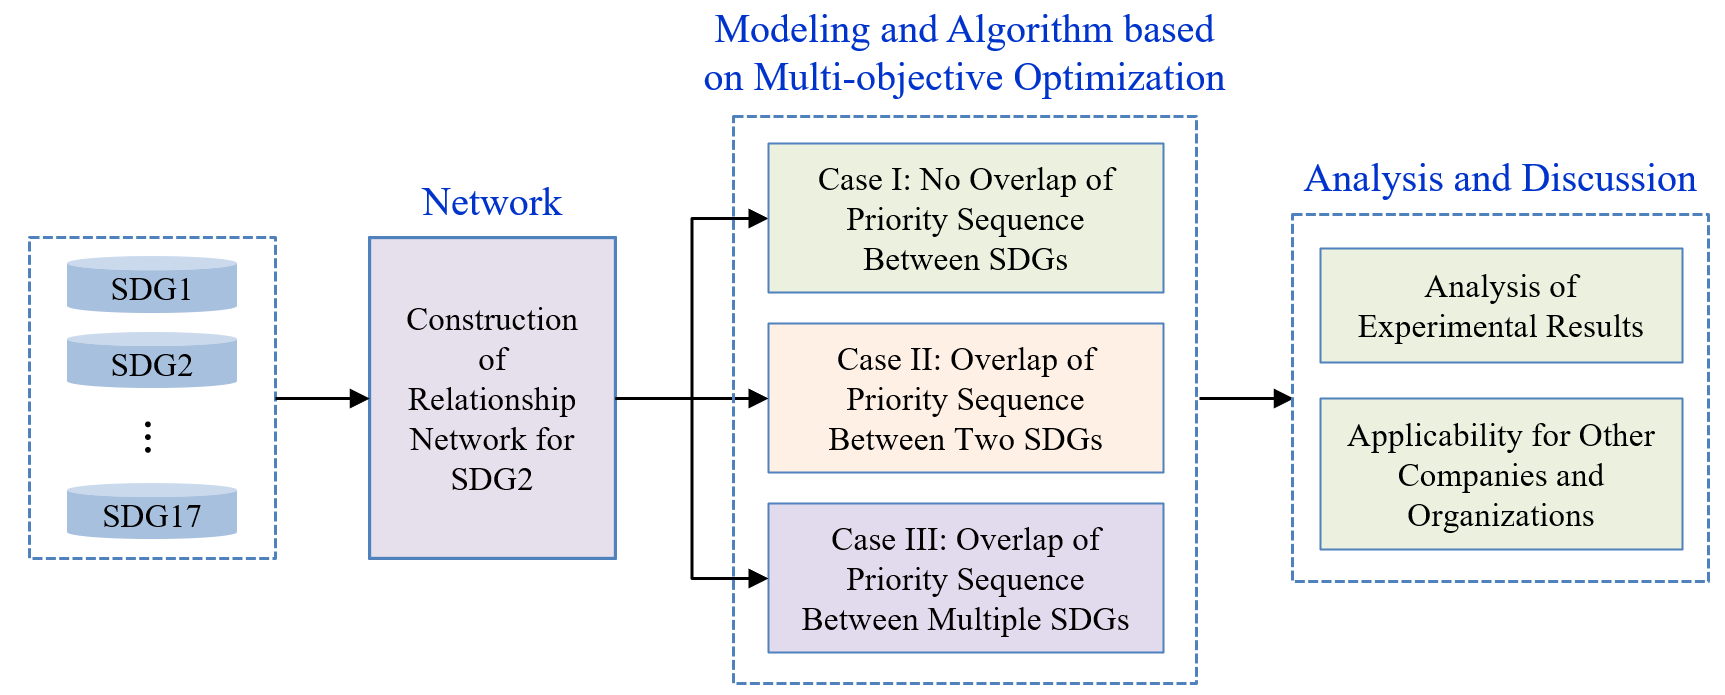
\includegraphics[width=16.0cm]{figures/road.png}
    \caption{ The flow chart }%后面加注释
    \label{fig.road}
\end{figure} 
\vspace{-25pt}


% 简单说一下
% 写一个ourwork,三个模型,分别多目标优化。
% 流程图 三个部分


% \emph{center of percussion} 



% %=======
% \begin{Theorem} \label{thm:latex}
% \LaTeX
% \end{Theorem}

% \begin{Lemma} \label{thm:tex}
% \TeX .
% \end{Lemma}

% \begin{proof}
% The proof of theorem.
% \end{proof}




\subsection{ Assumptions}
% 为了。。,做了如下假设
To build up our model, we make the following model assumptions:

% 	费用已知
% 	费用、时间的假设
% 	关联性的矩阵怎么做出来的  SDG-I数据对各个指标建立的模型是正确的
% 		时间相互依赖的矩阵 SDG-I数据能够反映各个指标的相关关系
% 	17项的权重  在所研究时期内,17项研究指标的权重是相同的
% 	相互依赖关系
% 		执行时间 执行成本和时间的转换关系可以简化为函数关系
% 		投资成本 投资每个SDGs的时间和资金仅随着策略顺序而变化
% 		关联关系可查
\begin{itemize}
%∙\bullet
\item  The weights of the 17 SGDs indicators were constant during the studied period.  \\

\item SDG-I data\cite{pradhan2017systematic}  can reflect the correlation of each indicator. \\

\item The execution time and investment money of each SDG varies with the priority sequence. That is, the values of the current SDG are affected by the SDGs that are positioned before the current SDG in the priority sequence.  \\

\item If a certain SDG has positive correlation values to some SDGs and it is positioned ahead of them in the priority sequence, the execution of this SDG will help to reduce the execution time and investment cost of the related SDGs.  \\
%仅考虑直接相连  一化,除以num

\end{itemize}




% The SDG-I\cite{pradhan2017systematic} aggregates the metrics associated with each of the 17 SDGs and arithmetically averages the results into one metric.
% 决策变量参数分开


% \subsection{ Notations}
% The key mathematical notations used in this paper are listed in Table ???????????????????????????????????????????????????????????????????????????????????????????????????????????????????????????????????????????????????????????????????????????????????????????????????????????????????????????????????????????????????????????????????????????????????????????????????????????????????????????????????????????????????????????????????????????????????????????????????????????????????????????????????????????????????????????????????????????????????????\ref{tab.notations}.
% 定义参数的表格
% \begin{table}[h]\caption{Notations used in this paper }
% % Please add the following required packages to your document preamble:
% % \usepackage{multirow}
% \small
% \centering
% \label{tab.notations}
% \begin{tabular}{cl}
% \hline
% Symbol                    & \multicolumn{1}{c}{Description}                                                      \\ \hline
% α\alpha                  & The upper bound                                                    \\ 
% Ki,jK_{i,j}                 & Degree of influence of task i and task j (facilitation or inhibit) \\ 
% CiC_i                     & Cost of performing task i                                          \\ 
% eie_i                     & Gain from performing task i                                        \\ 
% tit_i                     & Time required to perform task i                                    \\ 
% \multirow{2}{*}{xi,jx_{i,j}} & 1 when task i and task j are adjacent                              \\
%                           & 0 when task i and task j are not adjacent                          \\ 
% tit_i                     & Time required to perform task i   \\          
% Edi,jEd_{i,j}                &  Weight values of the one-way edges from i to j \\ \hline
% \end{tabular}
% \end{table}

% It follows that
% \begin{equation}\label{aa}
% a^2 + b^2 = c^2
% \end{equation}


% The equation (???)(???)(???)(???)(???)(???)(???)(???)(???)(???)(???)(???)(???)(???)(???)(???)(???)(???)(???)(???)(???)(???)(???)(???)(???)(???)(???)(???)(???)(???)(???)(???)(???)(???)(???)(???)(???)(???)(???)(???)(???)(???)(???)(???)(???)(???)(???)(???)(???)(???)(???)(???)(???)(???)(???)(???)(???)(???)(???)(???)(???)(???)(???)(???)(???)(???)(???)(???)(???)(???)(???)(???)(???)(???)(???)(???)(???)(???)(???)(???)(???)(???)(???)(???)(???)(???)(???)(???)(???)(???)(???)\eqref{aa} has told that

% \[
% \begin{pmatrix}
%   a_{11}  & a_{12}  & a_{13}   \\
%   a_{21}  & a_{22}  & a_{23}   \\
%   a_{31}  & a_{32}  & a_{33}
% \end{pmatrix}
% = \frac{{Opposite}}{{Hypotenuse}}\cos^{-1} \theta \arcsin \theta
% \]

% \[
% p_{j}=
% \begin{cases}
% 0,             & \text{if j is odd}\\
% r!\,(-1)^{j/2},& \text{if j is even}
% \end{cases}
% \]

% \[
% \arcsin \theta  = \oint\limits_\varphi \lim_{x \to \infty } \frac{n!}{r! (n - r)!} \eqno (23)
% \]












\section{Construction of Correlation Network for Sustainable Development Goals}

\subsection{ Literature review }
In this section, the existing literature is summarized in order to develop the network model. We chose the dataset after evaluating the practicability of the quantitative model.
\subsubsection{ Relationships between SDGs }
We provide a summary of recent research contributions evaluating potential relationships between SDGs. The results indicate that the relationships between the SDGs remain poorly understood \cite{allen2018initial}. There are instances in which the achievement of one SDG precludes progress on another, or where the achievement of one SDG is contingent on the achievement of another \cite{nilsson2016policy}. For instance, because poverty and inequality are reflected in consumption volumes \cite{aguiar2015has}, the progress made toward eradicating poverty (SDG1) and reducing inequalities (SDG10) could result in an increase in environmental impact. This is because most environmental effects can be directly and indirectly (via supply chains) attributed to household consumption \cite{ivanova2016environmental}.

Therefore, it is crucial to understand the relationships between SDGs and their scope and to recognize (or not) that a particular achievement may have positive or negative effects on other SDGs and their targets \cite{biggeri2019tracking}. The above work involves the correlation analysis of many indicators, but they focus on the qualitative analysis of only a few indicators.
The problem of constructing a relational network is transformed into finding the appropriate edge parameters for a directed graph with 17 nodes.

% \subsubsection{The global indicator framework}
% The global indicator framework for Sustainable Development Goals (GIF) was developed by the Inter-Agency and Expert Group on SDG Indicators (IAEG-SDGs) and ratified at the United Nations Statistical Commission's March 2017 48th session. The global indicator framework includes 231 unique indicators for 17 Sustainable Development Goals. Although these factors are essential guides for the 17 goals, the qualitative findings do not provide quantitative indicators.


\subsubsection{ The Sustainable Development Goal Index }
The Sustainable Development Goal Index (SDG-I) \cite{stiftung2018sustainable} aims to create and use a single, unified indicator for tracking progress toward the SDGs at the global level. It also aims to help identify priority action areas, track the overall development, and allow international comparisons and benchmarking\footnote{https://www.sdgindex.org/}.

The SDG-I relies on data from a variety of publicly accessible sources, encompassing all 193 United Nations member states since 2016. It is derived from a scoring system that uses the arithmetic mean to aggregate indicators for each of the 17 SDGs in turn, and then averages the results into a single metric \cite{biggeri2019tracking}. In order to reflect international commitments to treat each SDG equally and as an integrated and indivisible set of goals,a system of equal weights is consciously employed \cite{stiftung2018sustainable}. It has enormous potential (like other well-known composite indicators) for identifying action priorities, tracking overall progress, and conducting international comparisons.

\subsection{The Establishment of SDGs Correlation Network}
Several of the SDGs are difficult to convert into quantitative indicators owing to their conceptual complexity. 
In consideration of its worldwide validity and acceptability, the Sustainable Development Goal Index (SDG-I) \cite{pradhan2017systematic} was chosen as the data source for this research in order to circumvent these restrictions. 
The SDG-I aggregates indicators for each of the 17 Sustainable Development Goals and 'averages' the findings into a single statistic. 
In the data exploration phase, we follow the same method in \cite{fonseca2020mapping}.

% Taking into account the context and constraints, we must address the following questions.
By constructing a graph model to characterize the relationship between SDGs, we transform the problem into a graph node traversal order optimization problem, which can be modelled as a multi-objective optimization model to minimize total investment cost and execution time. Some details are as follows.


\subsubsection{ Kolmogorov-Smirnov Test}
Data on SDG-I\footnote{https://www.sdgindex.org/reports/sdg-index-and-dashboards-2018/} ranging from 2017 to 2022 is used in the following paragraph. An average score is calculated for every SDG. And the missing values in the data were supplemented by using linear differences.

To examine the normality of the data, the Kolmogorov-Smirnov Test was used, which is a non-parametric test used to determine whether data of a single sample follows a certain distribution or two samples of data come from the same distribution. The test is based on the comparison of the frequency distribution function $f(x)$ and the theoretical distribution function $g(x)$.The K-S test statistic $D$ is calculated as the maximum deviation between the two distribution functions. 
\begin{equation}
D=\max \left(\left|f(x)-g(x)\right|\right)
\end{equation}

The K-S test was applied to analyse the Sustainable Development Goal Index (SDG-I) of 17 SDGs for all 193 UN member states.The K-S normality test results of Table \ref{tab.Kolmogorov-Smirnov} showed that SDG 8, SDG 10, SDG 15 and SDG 16 don't follow a normal distribution considering that a $p$ value smaller than 0.05. Therefore, the correlation coefficient Spearman's Rho (which does not need normally distributed data and yields more reliable findings) was used.
\begin{table}[h]\caption{ Kolmogorov-Smirnov test results}
\tiny
\centering
\label{tab.Kolmogorov-Smirnov}
\tabcolsep=0.1cm
\begin{tabular}{llllllllllllllllll}
\hline
      & SDG1  & SDG2  & SDG3  & SDG4  & SDG5  & SDG6  & SDG7  & SDG8  & SDG9  & SDG10 & SDG11 & SDG12 & SDG13 & SDG14 & SDG15 & SDG16 & SDG17 \\ \hline
Stats & 0.322 & 0.073 & 0.140 & 0.166 & 0.105 & 0.131 & 0.215 & 0.051 & 0.135 & 0.065 & 1.260 & 0.149 & 0.172 & 0.132 & 0.035 & 0.060 & 0.087 \\ \hline
Sig.  & 0.000 & 0.042 & 0.000 & 0.000 & 0.000 & 0.000 & 0.000 & 0.200 & 0.000 & 0.200 & 0.000 & 0.000 & 0.000 & 0.000 & 0.200 & 0.200 & 0.000 \\ \hline
\end{tabular}
\end{table}


\subsubsection{Correlation Analysis  }
Spearman rank correlation coefficient, a non-parametric measure of the correlation between two variables, is used to assess the strength and direction of a monotonic relationship between two variables. Spearman's Rho $r_s$ based on the difference between two ranked variables is as follows:
\begin{equation}
r_s=1-\frac{6 \sum d_i^2}{N\left(N^2-1\right)}
\end{equation}

% 解释一下非对称权重怎么来的!!!!!!!!!!!!!!

The coefficient ranges from -1 to +1, where -1 indicates a perfect negative relationship between variables, 0 indicates no relationship, and +1 indicates a perfect positive relationship between two variables. The spearman rank correlation coefficient test was carried out with Python, where the overall results revealing several significant relationships between SDGs are presented in Table \ref{tab.adj ma}.



% 这边多补充一点
\begin{table}[!h]\caption{Adjacency Matrix of relevance}
\tabcolsep=0.1cm
\tiny
\label{tab.adj ma}  %//构建图的标签
\centering
\begin{tabular}{c|ccccccccccccccccc}
\hline
\textbf{}      & \textbf{SDG1}                                         & \textbf{SDG2}                                         & \textbf{SDG3}                                         & \textbf{SDG4}                                         & \textbf{SDG5}                                         & \textbf{SDG6}                                         & \textbf{SDG7}                                         & \textbf{SDG8}                                         & \textbf{SDG9}                                         & \textbf{SDG10}                                        & \textbf{SDG11}                                        & \textbf{SDG12}                                        & \textbf{SDG13}                 & \textbf{SDG14}                 & \textbf{SDG15}                 & \textbf{SDG16}                 & \textbf{SDG17}                 \\ \hline
\textbf{SDG1}  & \cellcolor[HTML]{F8DBB8}{\color[HTML]{000000} 1.000}  & \cellcolor[HTML]{F8DBB8}{\color[HTML]{000000} 0.609}  & \cellcolor[HTML]{F8DBB8}{\color[HTML]{000000} 0.734}  & \cellcolor[HTML]{F8DBB8}{\color[HTML]{000000} 0.670}  & \cellcolor[HTML]{F8DBB8}{\color[HTML]{000000} 0.338}  & \cellcolor[HTML]{F8DBB8}{\color[HTML]{000000} 0.357}  & \cellcolor[HTML]{F8DBB8}{\color[HTML]{000000} 0.661}  & \cellcolor[HTML]{F8DBB8}{\color[HTML]{000000} 0.578}  & \cellcolor[HTML]{F8DBB8}{\color[HTML]{000000} 0.686}  & \cellcolor[HTML]{F8DBB8}{\color[HTML]{000000} 0.424}  & \cellcolor[HTML]{F8DBB8}{\color[HTML]{000000} 0.466}  & \cellcolor[HTML]{F8DBB8}{\color[HTML]{000000} -0.570} & \cellcolor[HTML]{C7F8F6}-0.177 & \cellcolor[HTML]{C7F8F6}-0.007 & \cellcolor[HTML]{C7F8F6}-0.164 & \cellcolor[HTML]{C7F8F6}0.599  & \cellcolor[HTML]{C7F8F6}-0.103 \\
\textbf{SDG2}  & \cellcolor[HTML]{F8DBB8}{\color[HTML]{000000} 0.609}  & \cellcolor[HTML]{F8DBB8}{\color[HTML]{000000} 1.000}  & \cellcolor[HTML]{F8DBB8}{\color[HTML]{000000} 0.821}  & \cellcolor[HTML]{F8DBB8}{\color[HTML]{000000} 0.776}  & \cellcolor[HTML]{F8DBB8}{\color[HTML]{000000} 0.595}  & \cellcolor[HTML]{F8DBB8}{\color[HTML]{000000} 0.595}  & \cellcolor[HTML]{F8DBB8}{\color[HTML]{000000} 0.745}  & \cellcolor[HTML]{F8DBB8}{\color[HTML]{000000} 0.741}  & \cellcolor[HTML]{F8DBB8}{\color[HTML]{000000} 0.796}  & \cellcolor[HTML]{F8DBB8}{\color[HTML]{000000} 0.391}  & \cellcolor[HTML]{F8DBB8}{\color[HTML]{000000} 0.623}  & \cellcolor[HTML]{F8DBB8}{\color[HTML]{000000} -0.675} & \cellcolor[HTML]{C7F8F6}-0.095 & \cellcolor[HTML]{C7F8F6}0.170  & \cellcolor[HTML]{C7F8F6}0.042  & \cellcolor[HTML]{C7F8F6}0.590  & \cellcolor[HTML]{C7F8F6}-0.028 \\
\textbf{SDG3}  & \cellcolor[HTML]{F8DBB8}{\color[HTML]{000000} 0.734}  & \cellcolor[HTML]{F8DBB8}{\color[HTML]{000000} 0.821}  & \cellcolor[HTML]{F8DBB8}{\color[HTML]{000000} 1.000}  & \cellcolor[HTML]{F8DBB8}{\color[HTML]{000000} 0.857}  & \cellcolor[HTML]{F8DBB8}{\color[HTML]{000000} 0.612}  & \cellcolor[HTML]{F8DBB8}{\color[HTML]{000000} 0.501}  & \cellcolor[HTML]{F8DBB8}{\color[HTML]{000000} 0.840}  & \cellcolor[HTML]{F8DBB8}{\color[HTML]{000000} 0.784}  & \cellcolor[HTML]{F8DBB8}{\color[HTML]{000000} 0.892}  & \cellcolor[HTML]{F8DBB8}{\color[HTML]{000000} 0.372}  & \cellcolor[HTML]{F8DBB8}{\color[HTML]{000000} 0.711}  & \cellcolor[HTML]{F8DBB8}{\color[HTML]{000000} -0.789} & \cellcolor[HTML]{C7F8F6}-0.179 & \cellcolor[HTML]{C7F8F6}0.180  & \cellcolor[HTML]{C7F8F6}-0.053 & \cellcolor[HTML]{C7F8F6}0.736  & \cellcolor[HTML]{C7F8F6}-0.032 \\
\textbf{SDG4}  & \cellcolor[HTML]{F8DBB8}{\color[HTML]{000000} 0.670}  & \cellcolor[HTML]{F8DBB8}{\color[HTML]{000000} 0.776}  & \cellcolor[HTML]{F8DBB8}{\color[HTML]{000000} 0.857}  & \cellcolor[HTML]{F8DBB8}{\color[HTML]{000000} 1.000}  & \cellcolor[HTML]{F8DBB8}{\color[HTML]{000000} 0.655}  & \cellcolor[HTML]{F8DBB8}{\color[HTML]{000000} 0.542}  & \cellcolor[HTML]{F8DBB8}{\color[HTML]{000000} 0.773}  & \cellcolor[HTML]{F8DBB8}{\color[HTML]{000000} 0.731}  & \cellcolor[HTML]{F8DBB8}{\color[HTML]{000000} 0.811}  & \cellcolor[HTML]{F8DBB8}{\color[HTML]{000000} 0.341}  & \cellcolor[HTML]{F8DBB8}{\color[HTML]{000000} 0.712}  & \cellcolor[HTML]{F8DBB8}{\color[HTML]{000000} -0.705} & \cellcolor[HTML]{C7F8F6}-0.164 & \cellcolor[HTML]{C7F8F6}0.215  & \cellcolor[HTML]{C7F8F6}0.030  & \cellcolor[HTML]{C7F8F6}0.646  & \cellcolor[HTML]{C7F8F6}-0.018 \\
\textbf{SDG5}  & \cellcolor[HTML]{F8DBB8}{\color[HTML]{000000} 0.338}  & \cellcolor[HTML]{F8DBB8}{\color[HTML]{000000} 0.595}  & \cellcolor[HTML]{F8DBB8}{\color[HTML]{000000} 0.612}  & \cellcolor[HTML]{F8DBB8}{\color[HTML]{000000} 0.655}  & \cellcolor[HTML]{F8DBB8}{\color[HTML]{000000} 1.000}  & \cellcolor[HTML]{F8DBB8}{\color[HTML]{000000} 0.612}  & \cellcolor[HTML]{F8DBB8}{\color[HTML]{000000} 0.503}  & \cellcolor[HTML]{F8DBB8}{\color[HTML]{000000} 0.626}  & \cellcolor[HTML]{F8DBB8}{\color[HTML]{000000} 0.577}  & \cellcolor[HTML]{F8DBB8}{\color[HTML]{000000} 0.131}  & \cellcolor[HTML]{F8DBB8}{\color[HTML]{000000} 0.714}  & \cellcolor[HTML]{F8DBB8}{\color[HTML]{000000} -0.485} & \cellcolor[HTML]{C7F8F6}-0.083 & \cellcolor[HTML]{C7F8F6}0.223  & \cellcolor[HTML]{C7F8F6}0.061  & \cellcolor[HTML]{C7F8F6}0.313  & \cellcolor[HTML]{C7F8F6}0.116  \\
\textbf{SDG6}  & \cellcolor[HTML]{F8DBB8}{\color[HTML]{000000} 0.357}  & \cellcolor[HTML]{F8DBB8}{\color[HTML]{000000} 0.595}  & \cellcolor[HTML]{F8DBB8}{\color[HTML]{000000} 0.501}  & \cellcolor[HTML]{F8DBB8}{\color[HTML]{000000} 0.542}  & \cellcolor[HTML]{F8DBB8}{\color[HTML]{000000} 0.612}  & \cellcolor[HTML]{F8DBB8}{\color[HTML]{000000} 1.000}  & \cellcolor[HTML]{F8DBB8}{\color[HTML]{000000} 0.480}  & \cellcolor[HTML]{F8DBB8}{\color[HTML]{000000} 0.494}  & \cellcolor[HTML]{F8DBB8}{\color[HTML]{000000} 0.417}  & \cellcolor[HTML]{F8DBB8}{\color[HTML]{000000} 0.053}  & \cellcolor[HTML]{F8DBB8}{\color[HTML]{000000} 0.629}  & \cellcolor[HTML]{F8DBB8}{\color[HTML]{000000} -0.416} & \cellcolor[HTML]{C7F8F6}0.033  & \cellcolor[HTML]{C7F8F6}0.120  & \cellcolor[HTML]{C7F8F6}0.031  & \cellcolor[HTML]{C7F8F6}0.140  & \cellcolor[HTML]{C7F8F6}0.149  \\
\textbf{SDG7}  & \cellcolor[HTML]{F8DBB8}{\color[HTML]{000000} 0.661}  & \cellcolor[HTML]{F8DBB8}{\color[HTML]{000000} 0.745}  & \cellcolor[HTML]{F8DBB8}{\color[HTML]{000000} 0.840}  & \cellcolor[HTML]{F8DBB8}{\color[HTML]{000000} 0.773}  & \cellcolor[HTML]{F8DBB8}{\color[HTML]{000000} 0.503}  & \cellcolor[HTML]{F8DBB8}{\color[HTML]{000000} 0.480}  & \cellcolor[HTML]{F8DBB8}{\color[HTML]{000000} 1.000}  & \cellcolor[HTML]{F8DBB8}{\color[HTML]{000000} 0.611}  & \cellcolor[HTML]{F8DBB8}{\color[HTML]{000000} 0.785}  & \cellcolor[HTML]{F8DBB8}{\color[HTML]{000000} 0.291}  & \cellcolor[HTML]{F8DBB8}{\color[HTML]{000000} 0.655}  & \cellcolor[HTML]{F8DBB8}{\color[HTML]{000000} -0.673} & \cellcolor[HTML]{C7F8F6}-0.034 & \cellcolor[HTML]{C7F8F6}0.175  & \cellcolor[HTML]{C7F8F6}-0.061 & \cellcolor[HTML]{C7F8F6}0.572  & \cellcolor[HTML]{C7F8F6}0.050  \\
\textbf{SDG8}  & \cellcolor[HTML]{F8DBB8}{\color[HTML]{000000} 0.578}  & \cellcolor[HTML]{F8DBB8}{\color[HTML]{000000} 0.741}  & \cellcolor[HTML]{F8DBB8}{\color[HTML]{000000} 0.784}  & \cellcolor[HTML]{F8DBB8}{\color[HTML]{000000} 0.731}  & \cellcolor[HTML]{F8DBB8}{\color[HTML]{000000} 0.626}  & \cellcolor[HTML]{F8DBB8}{\color[HTML]{000000} 0.494}  & \cellcolor[HTML]{F8DBB8}{\color[HTML]{000000} 0.611}  & \cellcolor[HTML]{F8DBB8}{\color[HTML]{000000} 1.000}  & \cellcolor[HTML]{F8DBB8}{\color[HTML]{000000} 0.752}  & \cellcolor[HTML]{F8DBB8}{\color[HTML]{000000} 0.290}  & \cellcolor[HTML]{F8DBB8}{\color[HTML]{000000} 0.620}  & \cellcolor[HTML]{F8DBB8}{\color[HTML]{000000} -0.653} & \cellcolor[HTML]{C7F8F6}-0.164 & \cellcolor[HTML]{C7F8F6}0.193  & \cellcolor[HTML]{C7F8F6}-0.033 & \cellcolor[HTML]{C7F8F6}0.610  & \cellcolor[HTML]{C7F8F6}-0.159 \\
\textbf{SDG9}  & \cellcolor[HTML]{F8DBB8}{\color[HTML]{000000} 0.686}  & \cellcolor[HTML]{F8DBB8}{\color[HTML]{000000} 0.796}  & \cellcolor[HTML]{F8DBB8}{\color[HTML]{000000} 0.892}  & \cellcolor[HTML]{F8DBB8}{\color[HTML]{000000} 0.811}  & \cellcolor[HTML]{F8DBB8}{\color[HTML]{000000} 0.577}  & \cellcolor[HTML]{F8DBB8}{\color[HTML]{000000} 0.417}  & \cellcolor[HTML]{F8DBB8}{\color[HTML]{000000} 0.785}  & \cellcolor[HTML]{F8DBB8}{\color[HTML]{000000} 0.752}  & \cellcolor[HTML]{F8DBB8}{\color[HTML]{000000} 1.000}  & \cellcolor[HTML]{F8DBB8}{\color[HTML]{000000} 0.332}  & \cellcolor[HTML]{F8DBB8}{\color[HTML]{000000} 0.665}  & \cellcolor[HTML]{F8DBB8}{\color[HTML]{000000} -0.775} & \cellcolor[HTML]{C7F8F6}-0.208 & \cellcolor[HTML]{C7F8F6}0.240  & \cellcolor[HTML]{C7F8F6}0.002  & \cellcolor[HTML]{C7F8F6}0.741  & \cellcolor[HTML]{C7F8F6}-0.090 \\
\textbf{SDG10} & \cellcolor[HTML]{F8DBB8}{\color[HTML]{000000} 0.424}  & \cellcolor[HTML]{F8DBB8}{\color[HTML]{000000} 0.391}  & \cellcolor[HTML]{F8DBB8}{\color[HTML]{000000} 0.372}  & \cellcolor[HTML]{F8DBB8}{\color[HTML]{000000} 0.341}  & \cellcolor[HTML]{F8DBB8}{\color[HTML]{000000} 0.131}  & \cellcolor[HTML]{F8DBB8}{\color[HTML]{000000} 0.053}  & \cellcolor[HTML]{F8DBB8}{\color[HTML]{000000} 0.291}  & \cellcolor[HTML]{F8DBB8}{\color[HTML]{000000} 0.290}  & \cellcolor[HTML]{F8DBB8}{\color[HTML]{000000} 0.332}  & \cellcolor[HTML]{F8DBB8}{\color[HTML]{000000} 1.000}  & \cellcolor[HTML]{F8DBB8}{\color[HTML]{000000} 0.125}  & \cellcolor[HTML]{F8DBB8}{\color[HTML]{000000} -0.243} & \cellcolor[HTML]{C7F8F6}-0.070 & \cellcolor[HTML]{C7F8F6}-0.011 & \cellcolor[HTML]{C7F8F6}0.105  & \cellcolor[HTML]{C7F8F6}0.452  & \cellcolor[HTML]{C7F8F6}-0.065 \\
\textbf{SDG11} & \cellcolor[HTML]{F8DBB8}{\color[HTML]{000000} 0.466}  & \cellcolor[HTML]{F8DBB8}{\color[HTML]{000000} 0.623}  & \cellcolor[HTML]{F8DBB8}{\color[HTML]{000000} 0.711}  & \cellcolor[HTML]{F8DBB8}{\color[HTML]{000000} 0.712}  & \cellcolor[HTML]{F8DBB8}{\color[HTML]{000000} 0.714}  & \cellcolor[HTML]{F8DBB8}{\color[HTML]{000000} 0.629}  & \cellcolor[HTML]{F8DBB8}{\color[HTML]{000000} 0.655}  & \cellcolor[HTML]{F8DBB8}{\color[HTML]{000000} 0.620}  & \cellcolor[HTML]{F8DBB8}{\color[HTML]{000000} 0.665}  & \cellcolor[HTML]{F8DBB8}{\color[HTML]{000000} 0.250}  & \cellcolor[HTML]{F8DBB8}{\color[HTML]{000000} 1.000}  & \cellcolor[HTML]{F8DBB8}{\color[HTML]{000000} -0.608} & \cellcolor[HTML]{C7F8F6}-0.079 & \cellcolor[HTML]{C7F8F6}0.263  & \cellcolor[HTML]{C7F8F6}-0.026 & \cellcolor[HTML]{C7F8F6}0.450  & \cellcolor[HTML]{C7F8F6}0.097  \\
\textbf{SDG12} & \cellcolor[HTML]{F8DBB8}{\color[HTML]{000000} -0.570} & \cellcolor[HTML]{F8DBB8}{\color[HTML]{000000} -0.675} & \cellcolor[HTML]{F8DBB8}{\color[HTML]{000000} -0.789} & \cellcolor[HTML]{F8DBB8}{\color[HTML]{000000} -0.705} & \cellcolor[HTML]{F8DBB8}{\color[HTML]{000000} -0.485} & \cellcolor[HTML]{F8DBB8}{\color[HTML]{000000} -0.416} & \cellcolor[HTML]{F8DBB8}{\color[HTML]{000000} -0.673} & \cellcolor[HTML]{F8DBB8}{\color[HTML]{000000} -0.653} & \cellcolor[HTML]{F8DBB8}{\color[HTML]{000000} -0.775} & \cellcolor[HTML]{F8DBB8}{\color[HTML]{000000} -0.243} & \cellcolor[HTML]{F8DBB8}{\color[HTML]{000000} -0.608} & \cellcolor[HTML]{F8DBB8}{\color[HTML]{000000} 1.000}  & \cellcolor[HTML]{C7F8F6}0.324  & \cellcolor[HTML]{C7F8F6}-0.196 & \cellcolor[HTML]{C7F8F6}0.069  & \cellcolor[HTML]{C7F8F6}-0.570 & \cellcolor[HTML]{C7F8F6}0.029  \\
\textbf{SDG13} & \cellcolor[HTML]{C7F8F6}-0.177                        & \cellcolor[HTML]{C7F8F6}-0.095                        & \cellcolor[HTML]{C7F8F6}-0.179                        & \cellcolor[HTML]{C7F8F6}-0.164                        & \cellcolor[HTML]{C7F8F6}-0.083                        & \cellcolor[HTML]{C7F8F6}0.033                         & \cellcolor[HTML]{C7F8F6}-0.034                        & \cellcolor[HTML]{C7F8F6}-0.164                        & \cellcolor[HTML]{C7F8F6}-0.208                        & \cellcolor[HTML]{C7F8F6}-0.070                        & \cellcolor[HTML]{C7F8F6}-0.079                        & \cellcolor[HTML]{C7F8F6}0.324                         & \cellcolor[HTML]{C7F8F6}1.000  & \cellcolor[HTML]{C7F8F6}-0.012 & \cellcolor[HTML]{C7F8F6}0.179  & \cellcolor[HTML]{C7F8F6}-0.240 & \cellcolor[HTML]{C7F8F6}-0.018 \\
\textbf{SDG14} & \cellcolor[HTML]{C7F8F6}-0.007                        & \cellcolor[HTML]{C7F8F6}0.170                         & \cellcolor[HTML]{C7F8F6}0.180                         & \cellcolor[HTML]{C7F8F6}0.215                         & \cellcolor[HTML]{C7F8F6}0.223                         & \cellcolor[HTML]{C7F8F6}0.120                         & \cellcolor[HTML]{C7F8F6}0.175                         & \cellcolor[HTML]{C7F8F6}0.193                         & \cellcolor[HTML]{C7F8F6}0.240                         & \cellcolor[HTML]{C7F8F6}-0.011                        & \cellcolor[HTML]{C7F8F6}0.263                         & \cellcolor[HTML]{C7F8F6}-0.196                        & \cellcolor[HTML]{C7F8F6}-0.012 & \cellcolor[HTML]{C7F8F6}1.000  & \cellcolor[HTML]{C7F8F6}0.152  & \cellcolor[HTML]{C7F8F6}0.110  & \cellcolor[HTML]{C7F8F6}0.059  \\
\textbf{SDG15} & \cellcolor[HTML]{C7F8F6}-0.164                        & \cellcolor[HTML]{C7F8F6}0.042                         & \cellcolor[HTML]{C7F8F6}-0.053                        & \cellcolor[HTML]{C7F8F6}0.030                         & \cellcolor[HTML]{C7F8F6}0.061                         & \cellcolor[HTML]{C7F8F6}0.031                         & \cellcolor[HTML]{C7F8F6}-0.061                        & \cellcolor[HTML]{C7F8F6}-0.033                        & \cellcolor[HTML]{C7F8F6}0.002                         & \cellcolor[HTML]{C7F8F6}0.105                         & \cellcolor[HTML]{C7F8F6}-0.026                        & \cellcolor[HTML]{C7F8F6}0.069                         & \cellcolor[HTML]{C7F8F6}0.179  & \cellcolor[HTML]{C7F8F6}0.152  & \cellcolor[HTML]{C7F8F6}1.000  & \cellcolor[HTML]{C7F8F6}-0.014 & \cellcolor[HTML]{C7F8F6}-0.047 \\
\textbf{SDG16} & \cellcolor[HTML]{C7F8F6}0.599                         & \cellcolor[HTML]{C7F8F6}0.590                         & \cellcolor[HTML]{C7F8F6}0.736                         & \cellcolor[HTML]{C7F8F6}0.646                         & \cellcolor[HTML]{C7F8F6}0.313                         & \cellcolor[HTML]{C7F8F6}0.140                         & \cellcolor[HTML]{C7F8F6}0.572                         & \cellcolor[HTML]{C7F8F6}0.610                         & \cellcolor[HTML]{C7F8F6}0.741                         & \cellcolor[HTML]{C7F8F6}0.452                         & \cellcolor[HTML]{C7F8F6}0.450                         & \cellcolor[HTML]{C7F8F6}-0.570                        & \cellcolor[HTML]{C7F8F6}-0.240 & \cellcolor[HTML]{C7F8F6}0.110  & \cellcolor[HTML]{C7F8F6}-0.014 & \cellcolor[HTML]{C7F8F6}1.000  & \cellcolor[HTML]{C7F8F6}-0.101 \\
\textbf{SDG17} & \cellcolor[HTML]{C7F8F6}-0.103                        & \cellcolor[HTML]{C7F8F6}-0.028                        & \cellcolor[HTML]{C7F8F6}-0.032                        & \cellcolor[HTML]{C7F8F6}-0.018                        & \cellcolor[HTML]{C7F8F6}0.116                         & \cellcolor[HTML]{C7F8F6}0.149                         & \cellcolor[HTML]{C7F8F6}0.050                         & \cellcolor[HTML]{C7F8F6}-0.159                        & \cellcolor[HTML]{C7F8F6}-0.090                        & \cellcolor[HTML]{C7F8F6}-0.065                        & \cellcolor[HTML]{C7F8F6}0.097                         & \cellcolor[HTML]{C7F8F6}0.029                         & \cellcolor[HTML]{C7F8F6}-0.018 & \cellcolor[HTML]{C7F8F6}0.059  & \cellcolor[HTML]{C7F8F6}-0.047 & \cellcolor[HTML]{C7F8F6}-0.101 & \cellcolor[HTML]{C7F8F6}1.000  \\ \hline
\end{tabular}
\end{table}


By using the data of SDG-I from 2016 to 2022, we generate the time matrix in Table \ref{tab.time}.
% 对于我们影响关系定义部分,就是与顺序相关的投资成本与时间,要有一个小例子,比如只写4个SDG的顺序,然后说明一下后续投资成本与实施时间是如何与顺序相关的,比如:A->B-->C-->D,其中A同时也有虚线指向D,这样在计算D的时候,就需要同时考虑A和C的影响。
% 对于工作量固定的项目,项目执行时间和项目投资的关系满足经验公式:,我们因此可以由项目时间矩阵直接得到项目成本矩阵。
For projects with a fixed workload, the relationship between project execution time and project investment satisfies the empirical formula: $time = \cos{cost}$. We can therefore obtain the project cost matrix directly from the project time matrix.



\begin{table}[h]\caption{ Adjacency Matrix of time }
\tiny
\label{tab.time}
\tabcolsep=0.1cm
\centering
\begin{tabular}{c|ccccccccccccccccc}
\hline
      & SDG1   & SDG2   & SDG3   & SDG4   & SDG5   & SDG6   & SDG7   & SDG8   & SDG9   & SDG10  & SDG11  & SDG12  & SDG13  & SDG14  & SDG15  & SDG16  & SDG17  \\ \hline
SDG1  & 1.000  & 0.609  & 0.734  & 0.670  & 0.338  & 0.357  & 0.661  & 0.578  & 0.686  & 0.424  & 0.466  & -0.570 & -0.177 & -0.007 & -0.164 & 0.599  & -0.103 \\
SDG2  & 0.548  & 1.000  & 0.821  & 0.776  & 0.595  & 0.595  & 0.745  & 0.741  & 0.796  & 0.391  & 0.623  & -0.675 & -0.095 & 0.170  & 0.042  & 0.590  & -0.028 \\
SDG3  & 0.712  & 0.115  & 1.000  & 0.857  & 0.612  & 0.501  & 0.840  & 0.784  & 0.892  & 0.372  & 0.711  & -0.789 & -0.179 & 0.180  & -0.053 & 0.736  & -0.032 \\
SDG4  & 0.529  & 0.636  & -0.137 & 1.000  & 0.655  & 0.542  & 0.773  & 0.731  & 0.811  & 0.341  & 0.712  & -0.705 & -0.164 & 0.215  & 0.030  & 0.646  & -0.018 \\
SDG5  & 0.287  & -0.006 & -0.080 & -0.039 & 1.000  & 0.612  & 0.503  & 0.626  & 0.577  & 0.131  & 0.714  & -0.485 & -0.083 & 0.223  & 0.061  & 0.313  & 0.116  \\
SDG6  & -0.093 & -0.089 & 0.306  & 0.526  & 0.459  & 1.000  & 0.480  & 0.494  & 0.417  & 0.053  & 0.629  & -0.416 & 0.033  & 0.120  & 0.031  & 0.140  & 0.149  \\
SDG7  & 0.139  & 0.410  & 0.445  & 0.070  & 0.126  & 0.053  & 1.000  & 0.611  & 0.785  & 0.291  & 0.655  & -0.673 & -0.034 & 0.175  & -0.061 & 0.572  & 0.050  \\
SDG8  & 0.081  & 0.430  & 0.329  & 0.687  & -0.119 & 0.109  & -0.086 & 1.000  & 0.752  & 0.290  & 0.620  & -0.653 & -0.164 & 0.193  & -0.033 & 0.610  & -0.159 \\
SDG9  & 0.631  & 0.167  & 0.847  & 0.203  & 0.462  & -0.125 & 0.220  & 0.391  & 1.000  & 0.332  & 0.665  & -0.775 & -0.208 & 0.240  & 0.002  & 0.741  & -0.090 \\
SDG10 & 0.407  & 0.121  & -0.015 & 0.130  & 0.110  & 0.050  & 0.250  & 0.006  & 0.043  & 1.000  & 0.125  & -0.243 & -0.070 & -0.011 & 0.105  & 0.452  & -0.065 \\
SDG11 & 0.000  & 0.530  & 0.597  & 0.691  & -0.171 & 0.384  & 0.085  & -0.056 & 0.652  & 0.090  & 1.000  & -0.608 & -0.079 & 0.263  & -0.026 & 0.450  & 0.097  \\
SDG12 & 0.034  & -0.419 & -0.781 & -0.176 & 0.102  & -0.266 & -0.323 & -0.287 & 0.163  & -0.117 & -0.553 & 1.000  & 0.324  & -0.196 & 0.069  & -0.570 & 0.029  \\
SDG13 & -0.080 & 0.029  & -0.120 & 0.031  & 0.015  & 0.023  & 0.006  & -0.069 & -0.187 & 0.019  & -0.006 & 0.143  & 1.000  & -0.012 & 0.179  & -0.240 & -0.018 \\
SDG14 & -0.006 & -0.027 & 0.101  & 0.026  & 0.016  & 0.097  & 0.159  & 0.178  & 0.106  & -0.005 & 0.171  & -0.176 & -0.004 & 1.000  & 0.152  & 0.110  & 0.059  \\
SDG15 & -0.105 & 0.007  & -0.016 & 0.022  & 0.053  & 0.029  & 0.005  & -0.027 & 0.002  & 0.051  & -0.007 & 0.062  & 0.097  & -0.009 & 1.000  & -0.014 & -0.047 \\
SDG16 & -0.162 & 0.283  & 0.574  & 0.142  & 0.166  & 0.014  & 0.023  & 0.378  & 0.593  & 0.104  & -0.135 & -0.091 & -0.017 & 0.106  & -0.012 & 1.000  & -0.101 \\
SDG17 & -0.049 & -0.018 & -0.002 & -0.008 & 0.082  & -0.001 & 0.046  & -0.100 & 0.010  & -0.003 & 0.055  & 0.023  & -0.011 & 0.026  & -0.008 & -0.007 & 1.000  \\ \hline
\end{tabular}
\end{table}


% 强调是双向的 
% % 插入网络图片


\subsubsection{Network construction }

% 这里多放几个图
Using the clustering approach, the adjacency matrix is divided into two components. 
The first group is SDG1 to SDG12 with relatively higher weight shown in Figure \ref{picd}(Orange). The second group is SDG13 to SDG17 with a relatively lower weight shown in Figure \ref{picd}(Orange).

 \begin{figure}[H]
    \centering
    
    \subfloat[]{
        \label{picd}
        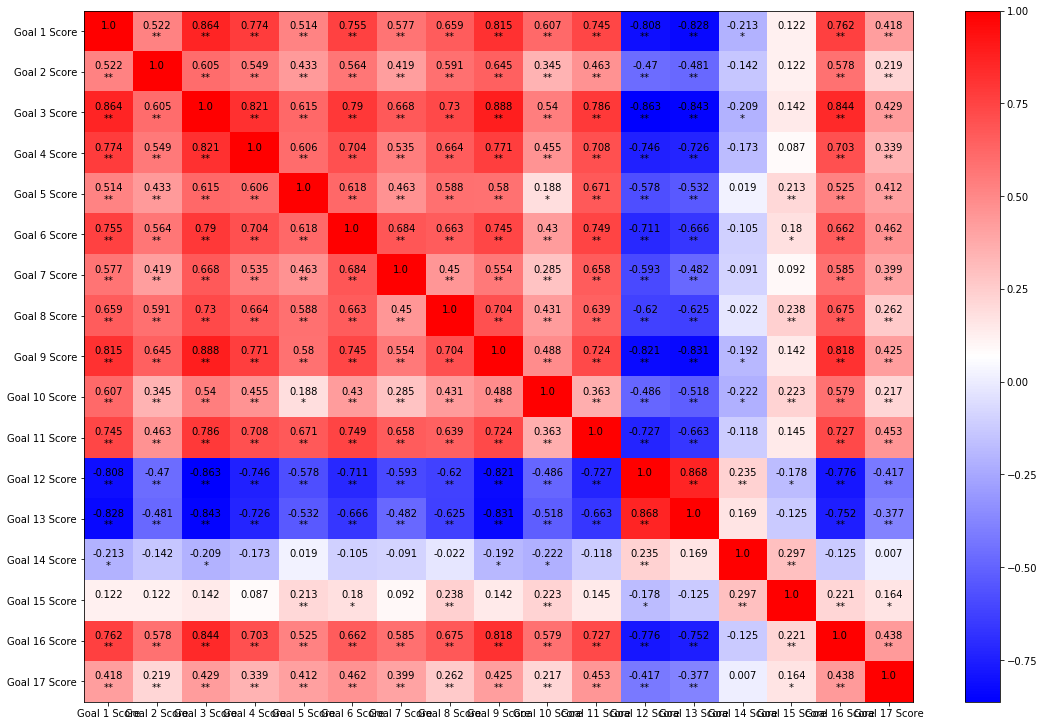
\includegraphics[width=7.0cm]{figures/mat_raw.png}
        % \caption{ Raw Matrix}
    }
    \subfloat[]{
        \label{picb}
        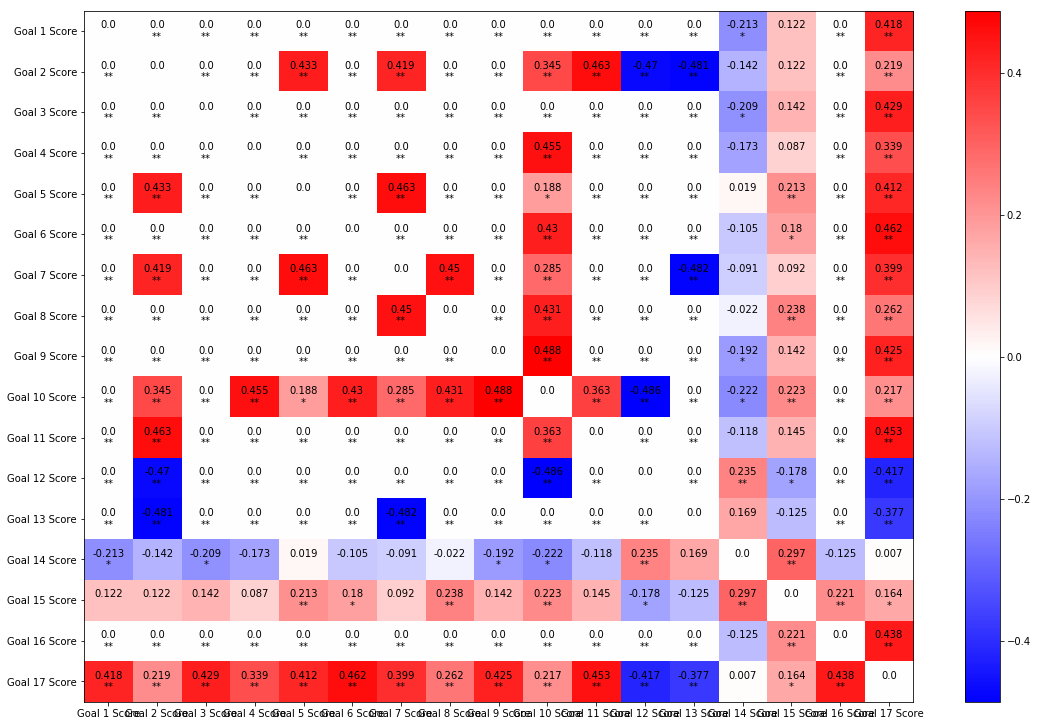
\includegraphics[width=7.0cm]{figures/mat_process.png}
        % \caption{After using the threshold }
    }
    \caption{ Visual comparison between the adjacency matrix map and enhanced adjacency matrix  }%修一下,不能两行
    \label{fig.compare}
\end{figure}
%1-12阈值为+-0.75
% 13-17阈值为+-0.4

Moreover, we establish two sets of threshold values to eliminate superfluous connections, which is shown in  Table \ref{tab.cons}. 
We further attenuated the tabular parameters according to the level of correlation coefficients to avoid dense connections between nodes. The result is shown in Figure \ref{picb}. Our thresholds take into account the correlation level and the upper alpha quantile and yield reliable results in the model.

\begin{table}[h]\caption{Constrain Parameter}
% Please add the following required packages to your document preamble:
% \usepackage{multirow}
\small
\centering
\label{tab.cons}
\begin{tabular}{cccc}
\hline
SDG number &    Symbol      & \multicolumn{1}{c}{Threshold}   & Color                                                   \\ \hline
1-12 &   $C_{dense}$           & $\pm 0.78$      & red                                             \\ 
13-17     &     $C_{sparce}$            &$\pm 0.4$ & blue   \\ \hline
\end{tabular}
\end{table}

The network is based on a graph theory approach\cite{beineke1997graph} to network analysis, applying community detection to identify indicators that are related to the network. The most significant core indicators were identified with the application node centrality metric in the network. Using the 17 UN Sustainable Development Goals (SDGs) as 17 nodes, the relationships between sustainable development goals were quantified. The magnitude of the relationships was defined as the width attribute of the edges. Meanwhile, the impact having a positive or negative effect was used as the colour attribute of the edges to gain insight into the network structure and properties.


% \subsection{}
%在第2节网络结构的后面,加一个小节,给一个小例子,比如4个节点,说明一下相邻关系对于投资成本和时间的影响

\begin{figure}[H]
    \centering
    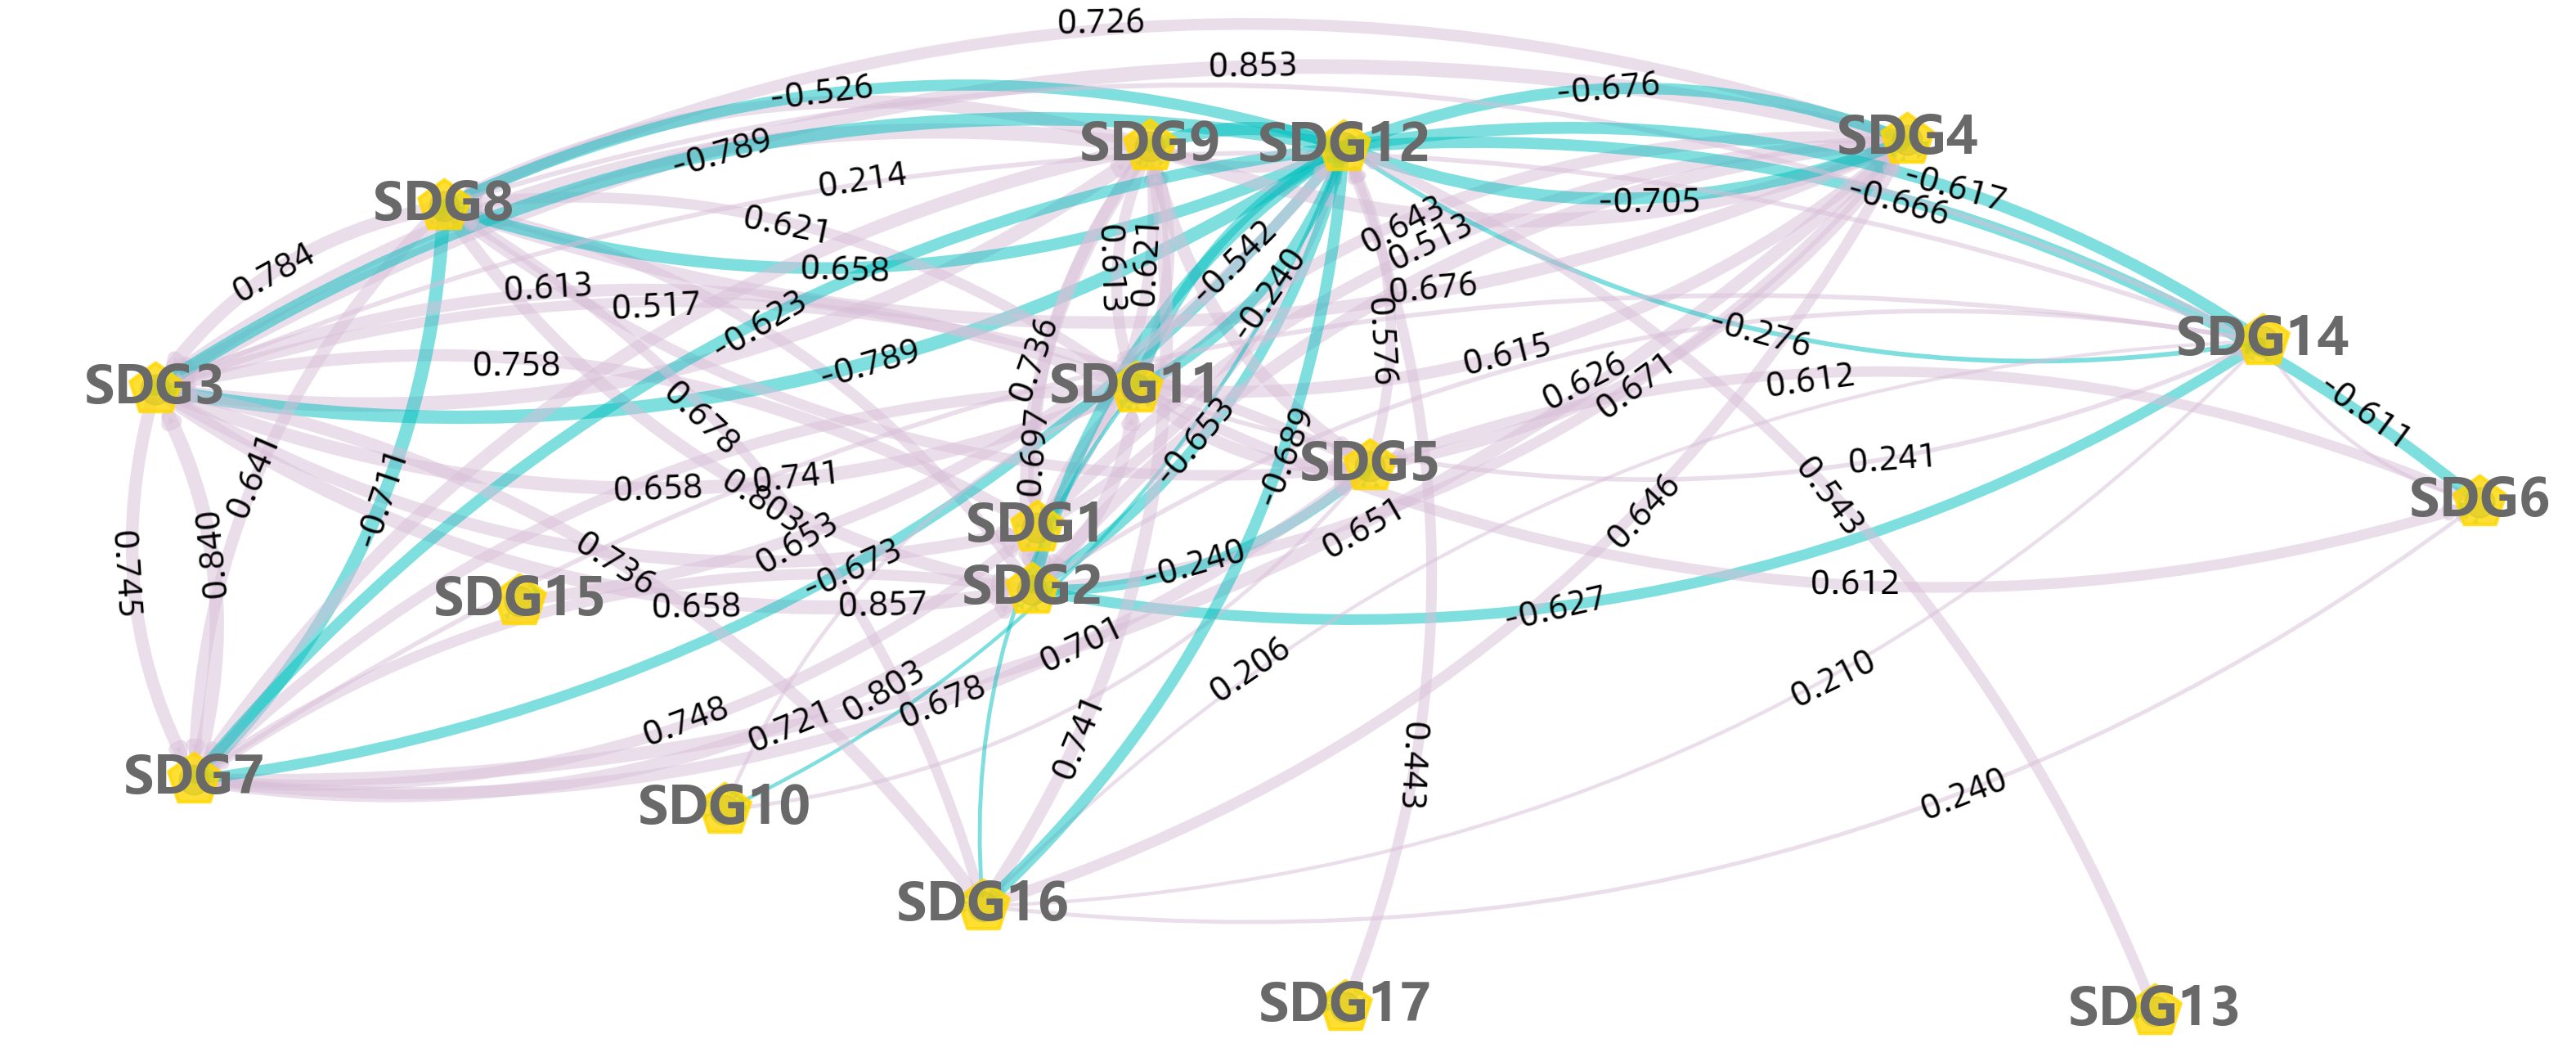
\includegraphics[width=14.0cm]{figures/modify_map.png}
    \caption{ Directed graph of 17 SDGs }%后面加注释
    \label{fig.graph}
\end{figure} 
\vspace{-15pt}

In this network graph, thistle edges represent positive influences between nodes, while dark turquoise edges represent negative influences between nodes. The width of the edges is set to 10 times the corresponding influence coefficients.

% 时间的顺序相关性
% 	目标函数就依赖这个
% 		给例子说一下,简单的,画个abcd,bd虚线
% 		ac虚线
% 		其他实线
% 		说明时间成本计算是顺序依赖的
% 		最后计算一下D,体现顺序依赖的计算方法,



 % \subsection{The Model Results}
%统计结果
% 由于数据分布非正态,不能简单的利用分位数。因此考虑到聚类算法,分为高度相关、相关度有限两类情况。


\section{Case I: Modeling without overlap}
% 介绍overlap
The scheduling problem is usually faced with the following two problems: overlapping activities and sequence-dependent setup cost. The models designed with and without overlap are quite different\cite{overlap1997}. 

Therefore we will start with the simplifying assumption that each SDGs can only be executed sequentially in turn. The model that is closer to the real situation and more complex will be given in the next chapter.



%\subsection{ Solution Evaluation}%1 针对case 定义的解的评价
% 1 针对case one定义的解的评价
% 	给例子
% 	画图
% 		权重系数写上
% 	重点说
% 	创新点??


\subsection{Mathematical Models based on Multi-objective Optimization}%2 参数、变量、目标、模型

\subsubsection{Parameters and Variables}

To build up our model, we make the following parameters and variables, as shown in Table \ref{tab.parameters} and Table \ref{tab.variables}.
Supposing $\mathrm{T}=\left\{0, 1, 2, \ldots, n\right\} $
is the set of n development projects and $\pi=[\pi(1), \pi(2), \ldots, \pi(n)]  $is an ordering of all projects. A dummy SDG indexed by 0 is incorporated to ensure the constraint that each SDG i has a previous and a subsequent SDG.

\begin{table}[!h]\caption{Parameters}
\small
\centering
\begin{tabular}{cl}
 \hline
\centering
\label{tab.parameters}
Symbol & \multicolumn{1}{c}{Description}                                                            \\ \hline
$n$     & total number of SDGs                                     \\
$r_{i j}$     & degree of impact (facilitation OR disincentive) of SDG $i$ and SDG $j$ \\
$C_i$    & base cost required to implement SDG $i$                                  \\
$t_i$     & basic time required to implement SDG $i$                                \\ \hline
\end{tabular}
\end{table}

\begin{table}[!h]\caption{ Decision-making variables}
\small
\centering
\label{tab.variables}
\begin{tabular}{cl}
 \hline
\centering
Symbol & \multicolumn{1}{c}{Description}                                                            \\ \hline
$p_i$     & actual time taken to execute SDG $i$                                                                                             \\
$s_i$     & start time of project $i$                                                                                                          \\
$e_i$     & the end time of project $i$                                                                                                        \\
$x_{i j}$     & \begin{tabular}[c]{@{}l@{}}1 - SDG $i$  and SDG $j$  are adjacent\\ 0 - SDG $i$ and SDG $j$ are not adjacent\end{tabular}
\\ \hline
\end{tabular}
\end{table}


\subsubsection{Objective Functions}

Minimisation of total execution time of all SDGs:

\begin{equation}
f_1= \min e_{\pi(n)}
\end{equation}

Minimization of total investment cost:

\begin{equation}
f_2=\min \sum_{j=1}^n(1-\sum_{i=1}^n r_{i j} \times x_{i j} / \sum_{j=1}^n x_{i j}) \times C_{j} \quad(i, j=1,2, \ldots, n ; i \neq j)
\end{equation}

\subsubsection{Constraints}
The priority sequence should start and end at the dummy SDG 00 :

\begin{equation}
    	\sum_{i=1}^nx_{0i}=\sum_{i=1}^nx_{i0}=1
\end{equation}

There is a SDG before and after each SDG i :
\begin{equation}
    	\sum_{j=0}^nx_{ij}=\sum_{j=0}^nx_{ji}=1, \quad(i=1,2, \ldots, n)
\end{equation}

The start time of the first SDG is 0:
\begin{equation}
s_{\pi(1)}=0
\end{equation}

The completion time of the first SDG is the same as the base time:
\begin{equation}
e_{\pi(1)}=t_{\pi(1)}
\end{equation}

The completion time of SDG $\pi(i)$  is:

\begin{equation}
e_{\pi(i)}=s_{\pi(i)}+p_{\pi(i)}, \quad(i=1,2, \ldots, n)
\end{equation}

SDG j cannot be started unless its previous SDG i has finished (MM is a very big number):
\begin{equation}
s_j \geq e_i+(x_{ij}-1)M, \quad(i, j=1,2, \ldots, n ; i \neq j)
\end{equation}

The actual execution time taken for SDG $\pi(i) $is affected by the SDG completed before it:
\begin{equation}
p_{\pi(i)}=(1-\sum_{j=1}^n r_{i j} \times x_{i j}/ \sum_{j=1}^n x_{i j}) \times t_{\pi(i)}, \quad(i, j=1,2, \ldots, n ; i \neq j)
\end{equation}

The completion time of each SDG is greater than 0:
\begin{equation}
e_i>0, \quad(i=1,2, \ldots, n)
\end{equation}



% 2 参数、变量、目标、模型
% 	时间表、各类参数怎么得到的

% 17个权重 
The weights of 17 SDGs were calculated by applying AHP to the analysis of all 102 countries with the 17 SDGs as the indicators.
Analytic Hierarchy Process\cite{torfi2010fuzzy} is a structured approach to decision-making developed by mathematician and operations researcher Thomas Saaty in the 1970s. We constructed a judgement matrix by using the data of SDG index and then corrected it with a consistency test. The judgement matrix was used to calculate the relative weights using the arithmetic mean method finally. The detailed function is listed in Appendix \ref{code.ahp}.


% \subsubsection{ Relationship in Time}

\subsection{Decomposition-based multi-objective evolutionary algorithm (MOEA/D)}

MOEA/D is a population-based evolutionary algorithm widely used for solving complex multi-objective optimization problems due to its superior search performance. Its basic idea is to partition the search space into a set of regions called 'sub-regions' and to correspondingly solve a subproblem in each sub-region, thereby transforming a multi-objective optimization problem into multiple subproblems. In addition, the MOEA/D algorithm proceeds in a decomposed manner at each step, i.e., performing single-objective optimization in each sub-region and then collaborating among subproblems to achieve an approximate Pareto optimal solution. In the MOEA/D algorithm, all sub-regions are determined by a set of user-predefined reference points (i.e., target vectors uniformly distributed in the space). The number of reference points can be customized and remains unchanged during the optimization process, thus ensuring that the MOEA/D algorithm can find high-quality candidate solutions in each iteration.

\subsubsection{Overall framework of MOEA/D}
The flowchart of the MOEA/D algorithm is given in Figure \ref{fig.moead}, and its main processes are described as follows.

    1) First, initialize the population and the uniformly distributed weight vector. Set the algorithm stopping criterion.
    
    2) For each weight vector $\lambda_{i}$, the nearest $T$ vectors in the target space are taken as neighbors, denoted as $B(i)$.
    
    3) Calculate the initial population objective function and set the ideal point $z$.
    
    4) For each individual x in the population, generate a new solution y according to the genetic operator.
    
    5) Update the ideal point $z$ and the neighborhood of solution x according to the solution y.
    
    6) Determine whether the stopping criterion is satisfied, and if so the algorithm stops. Otherwise, return to step (4).


\begin{figure}[H]
    \centering
    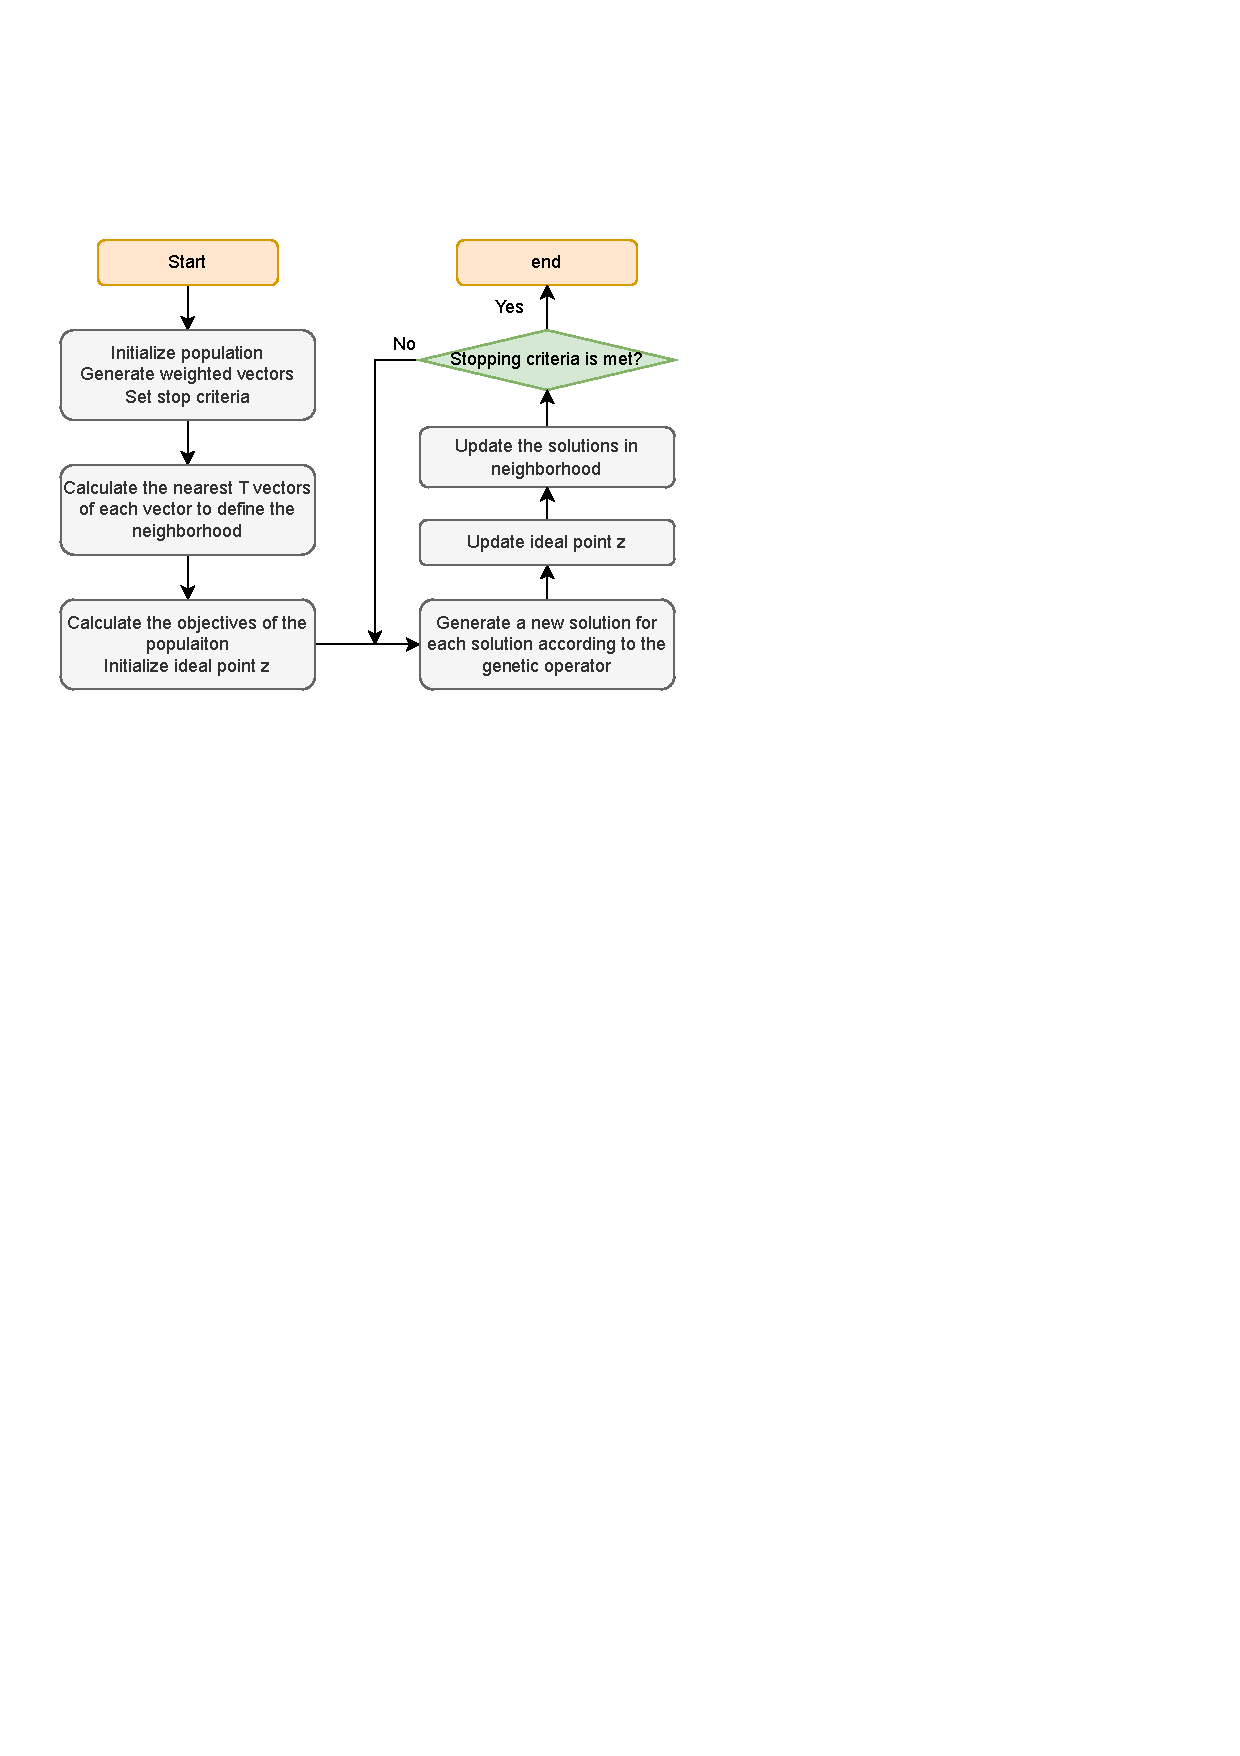
\includegraphics[width=7.0cm]{figures/Moead.pdf}
    \caption{ Flowchart of MOEA/D Algorithm }%后面加注释
    \label{fig.moead}
\end{figure} 
\vspace{-15pt}


\subsubsection{Encoding Mechanism}

In the process of iterative evolution of the algorithm, it is necessary to establish a mapping relationship between the chromosome and the execution plan. Considering the characteristics of combinatorial optimization problems, this paper adopts Permutation encoding, where the length of the chromosome is the same as the number of tasks to be executed. The $i^{th}$  gene value $s_i  (i=1,2,...,n) (i = 1, 2, ..., n) $ on the chromosome represents that the $i^{th}$ task to be executed is $s_i$, where n is the length of the chromosome. In addition, feasible chromosomes must satisfy the condition that all gene values are unique. The encoding diagram is shown in Figure \ref{fig.noover}.

\begin{figure}[H]
    \centering
    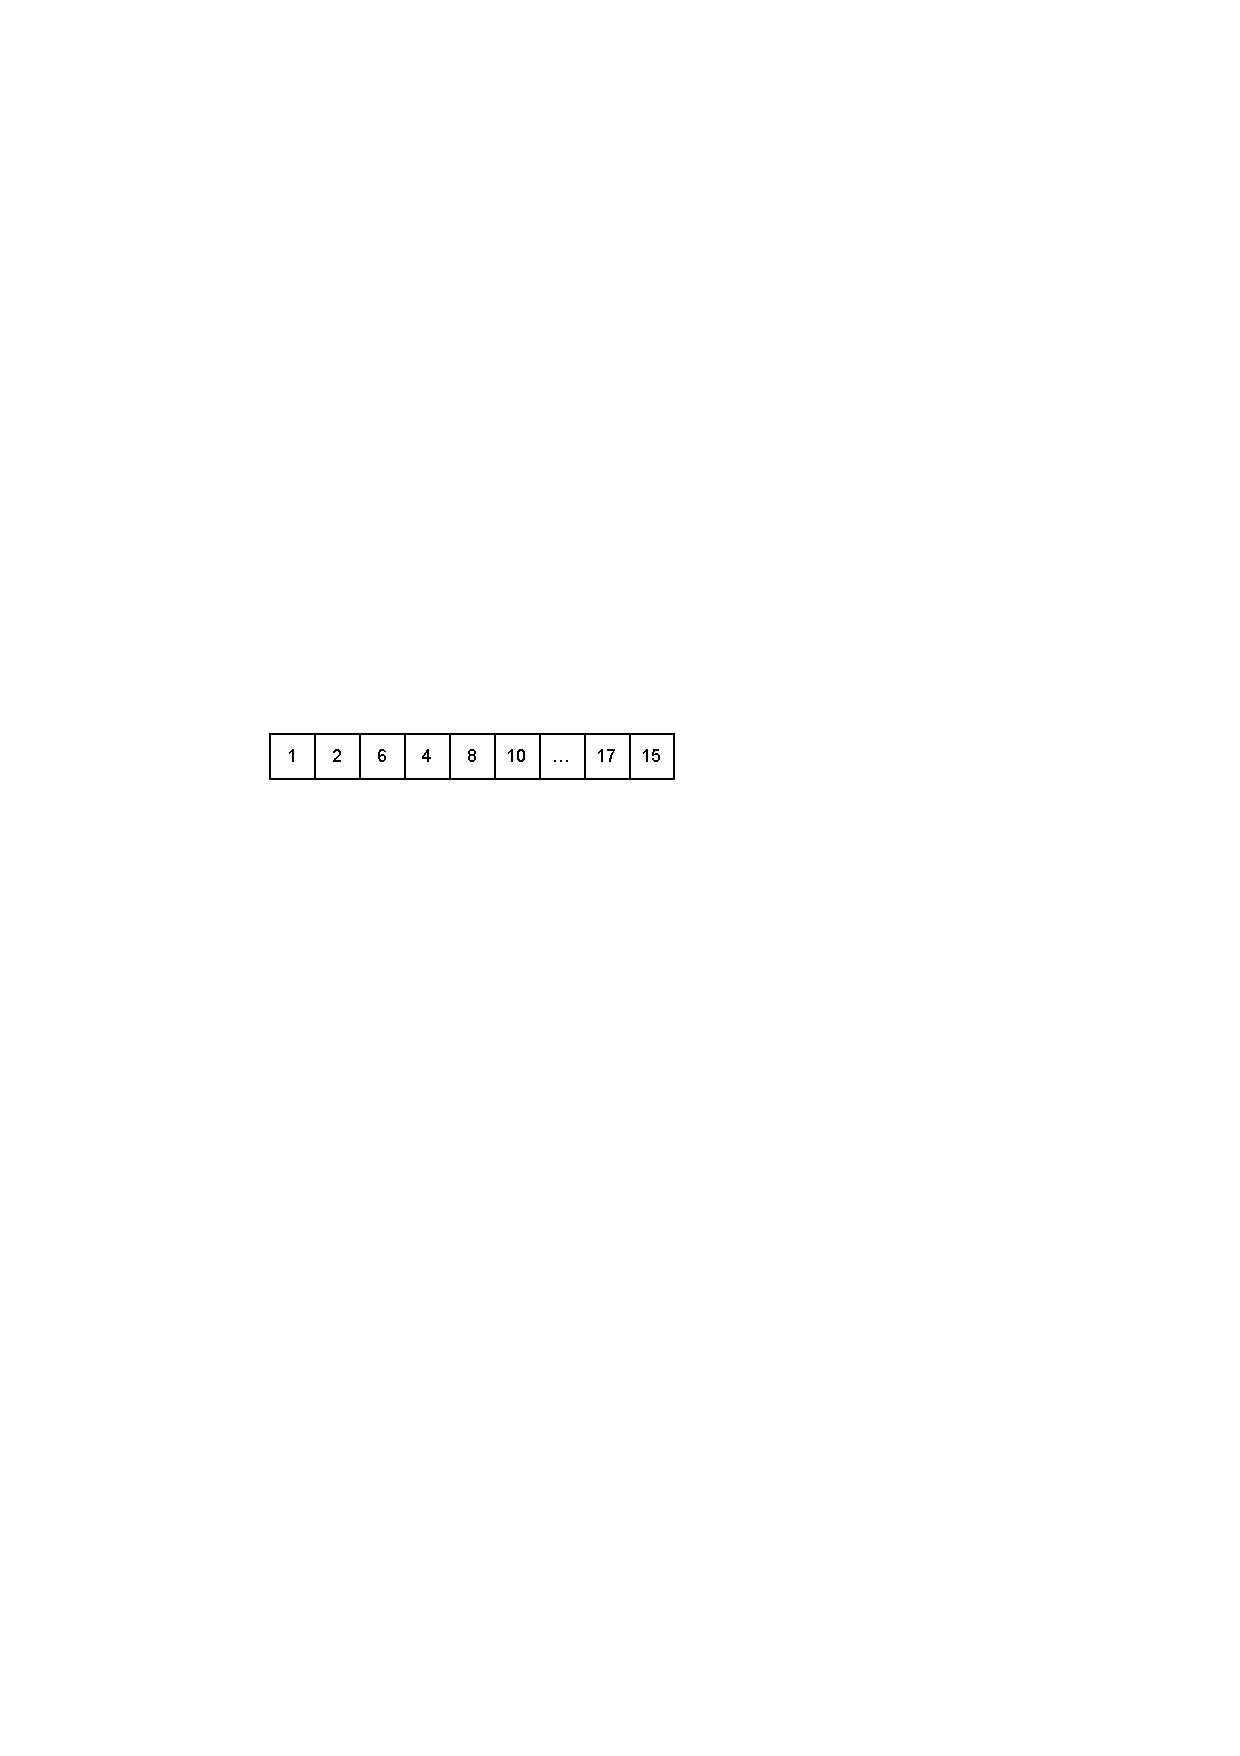
\includegraphics[width=7.0cm]{figures/NoOverlap.pdf}
    \caption{ Encoding diagram without Overlap }%后面加注释
    \label{fig.noover}
\end{figure} 
\vspace{-15pt}

% \begin{figure}[H]
%     \centering
%     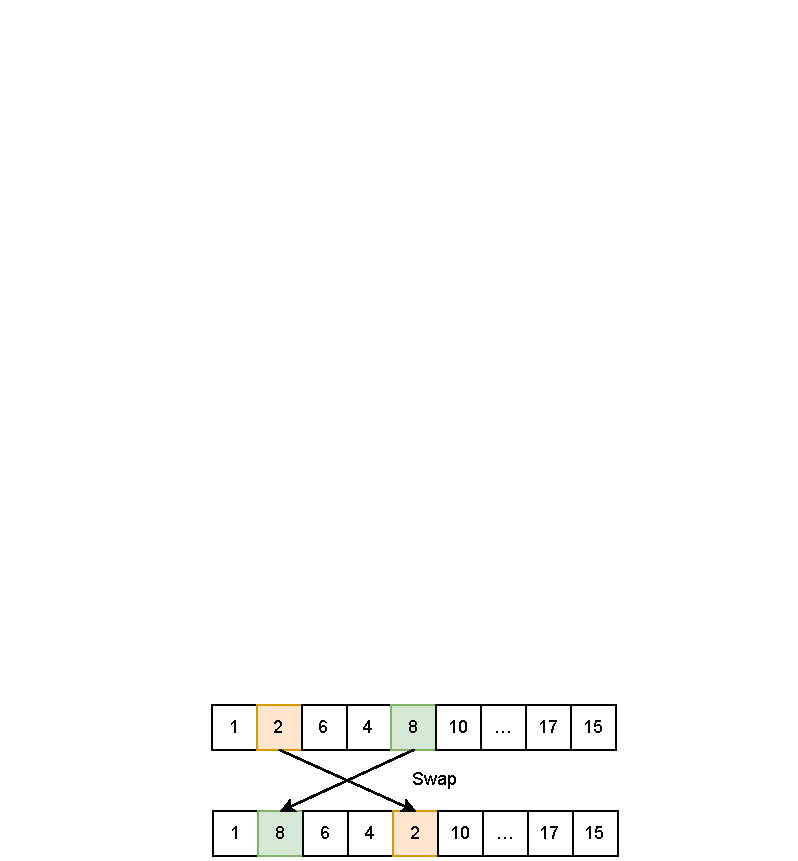
\includegraphics[width=7.0cm]{figures/Swap.pdf}
%     \caption{ Encoding diagram }%后面加注释
%     \label{fig.swap}
% \end{figure} 
% % Figure 2 and 3: Chromosome encoding diagrams

\subsubsection{Crossover operator to generate new solutions}

The crossover operator is an important part of evolutionary algorithms. Using a crossover operator that is suitable for the problem characteristics can not only improve the search ability of the algorithm but also accelerate the convergence speed and effectively improve the algorithm's solving performance. Since the task execution optimization problem studied in this paper can be reduced to a discrete optimization problem, the commonly used Swap mutation method for permutation-type problems is adopted. The Swap mutation diagram is shown in Figure \ref{fig.cross}.

\begin{figure}[H]
    \centering
    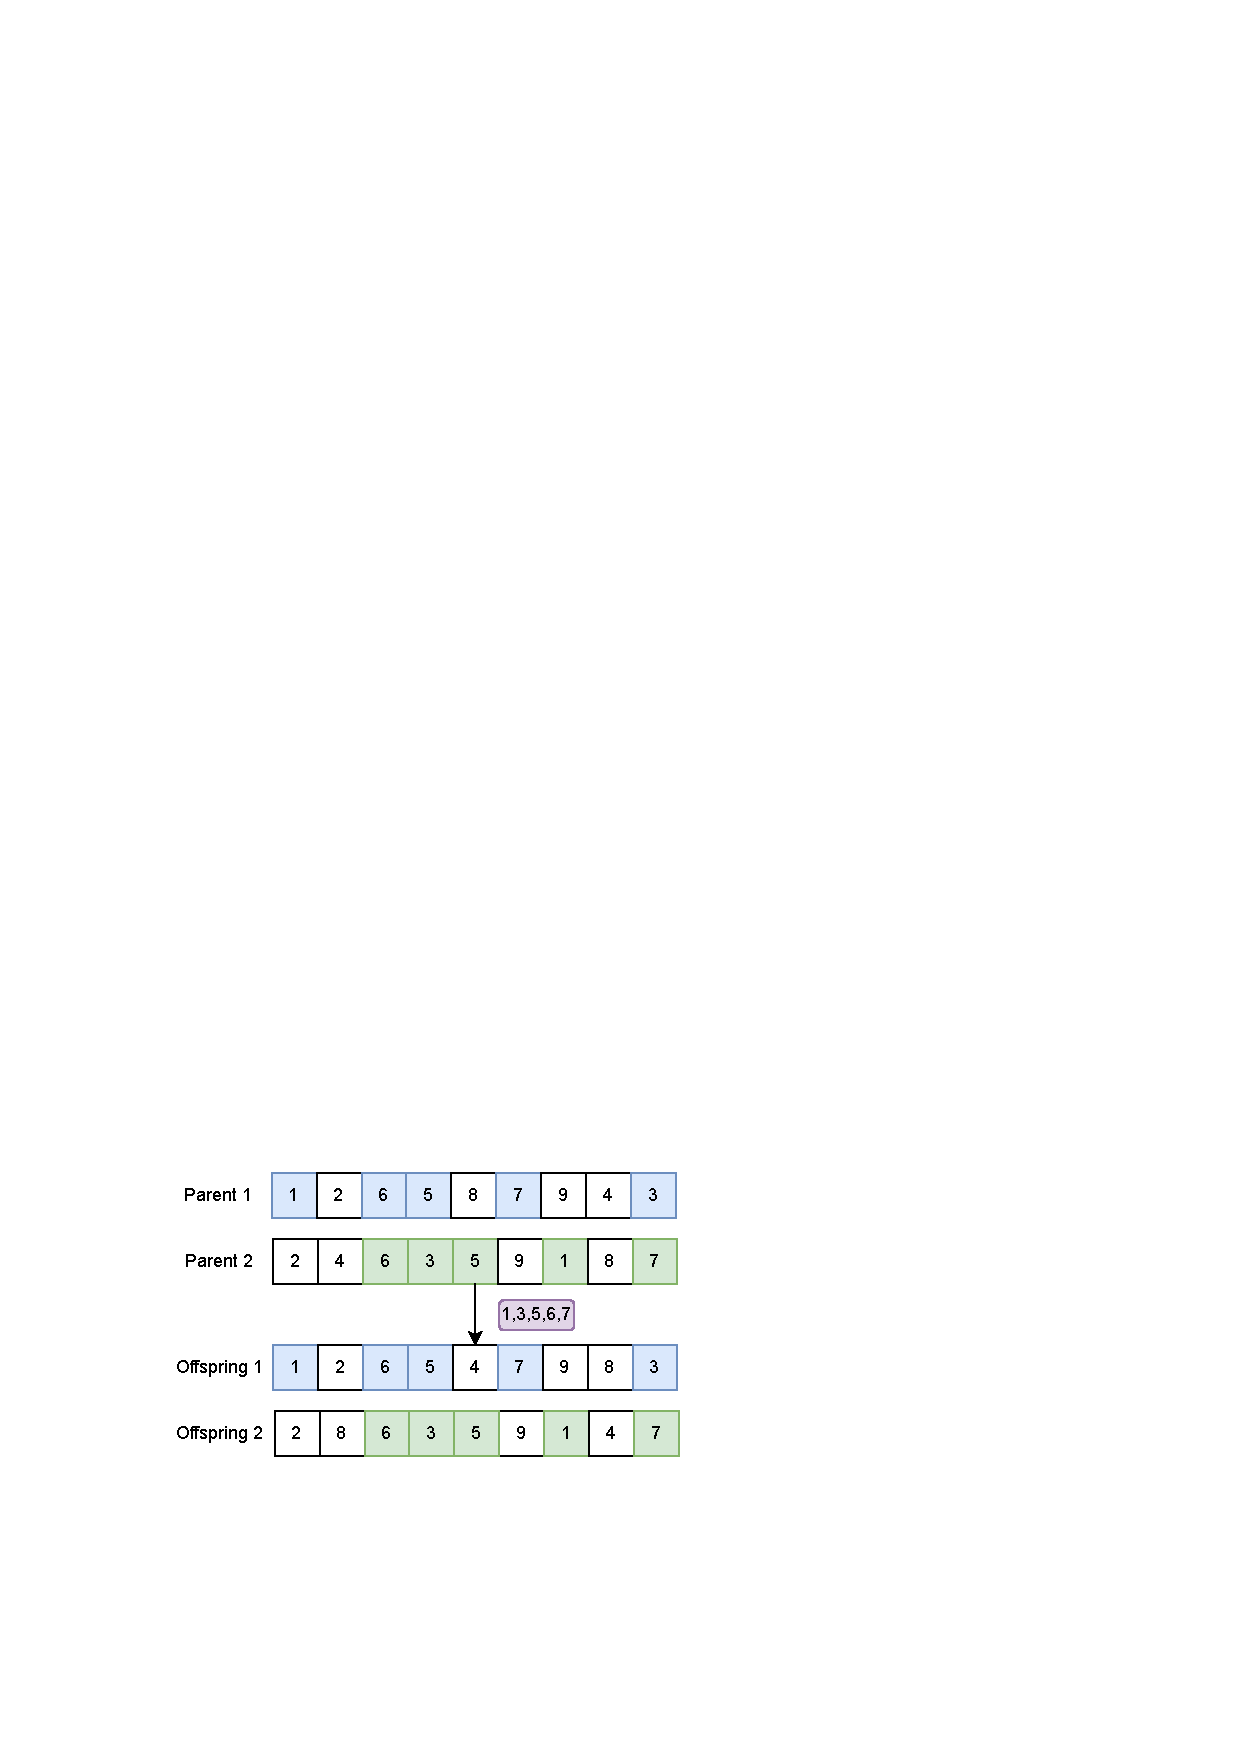
\includegraphics[width=7.0cm]{figures/cross_over.pdf}
    \caption{ Cross over }%后面加注释
    \label{fig.cross}
\end{figure} 
\vspace{-15pt}
% Figure 4: Swap mutation diagram

\subsubsection{ Evaluation of a solution considering the effectiveness of each priority}
% 在我们的模型中,时间花费将随着任务顺序改变而变化。 比如在SDG1,SDG3,SDG6,SDG9四个样本中,他们的连接关系如图所示。
In our model, the time spent will change as the task order changes. For example, in the four samples of SDG1, SDG3, SDG6, and SDG9, their connection relationship is shown in Fig \ref{fig.example}. 
% 图a展示了时间相关性中简单的设置,所有的节点由固定的数值连接。这意味着不论何时运行此SDG,算法得到的增益都是定值。而我们的模型对顺序进行了良好的建模,使得所耗费的时间和资金成本取决于遍历节点的顺序。
Figure \ref{pic1} shows a simple setup in time correlation where all the nodes are connected by a fixed value. This means that the gain obtained by the algorithm is a fixed value regardless of when this SDG is run. And our model models(fig \ref{pic2}) the order well, so that the time and money cost spent depends on the order of traversing the nodes.

% 考虑发展顺序序列SDG1, SDG3, SDG6。 在图a的设置中,此序列的时间恒定为T_1+T_3+T_6,数值不随着顺序变化。 在图b设置中,时间为T_{1,1}+T_{1,3}+T_{3,6},是顺序相关的。
Consider the development of sequential sequences SDG1, SDG3, SDG6. In the setup of Fig. a, the time of this sequence is constant as$ T_1+T_6$ and the values do not change with the order. In the setup of Figure b, the time is $T_{1,1}+T_{1,3}+T_{3,6}$, which is sequentially correlated. 
% 这个问题的回答放到算法的解的编码之后,就是对解的评价,给一个例子,说明一下怎么算的
% 对于我们影响关系定义部分,就是与顺序相关的投资成本与时间,要有一个小例子,比如只写4个SDG的顺序,然后说明一下后续投资成本与实施时间是如何与顺序相关的,比如:A->B-->C-->D,其中A同时也有虚线指向D,这样在计算D的时候,就需要同时考虑A和C的影响。

 \begin{figure}[H]
    \centering
    
    \subfloat[]{
        \label{pic1}
        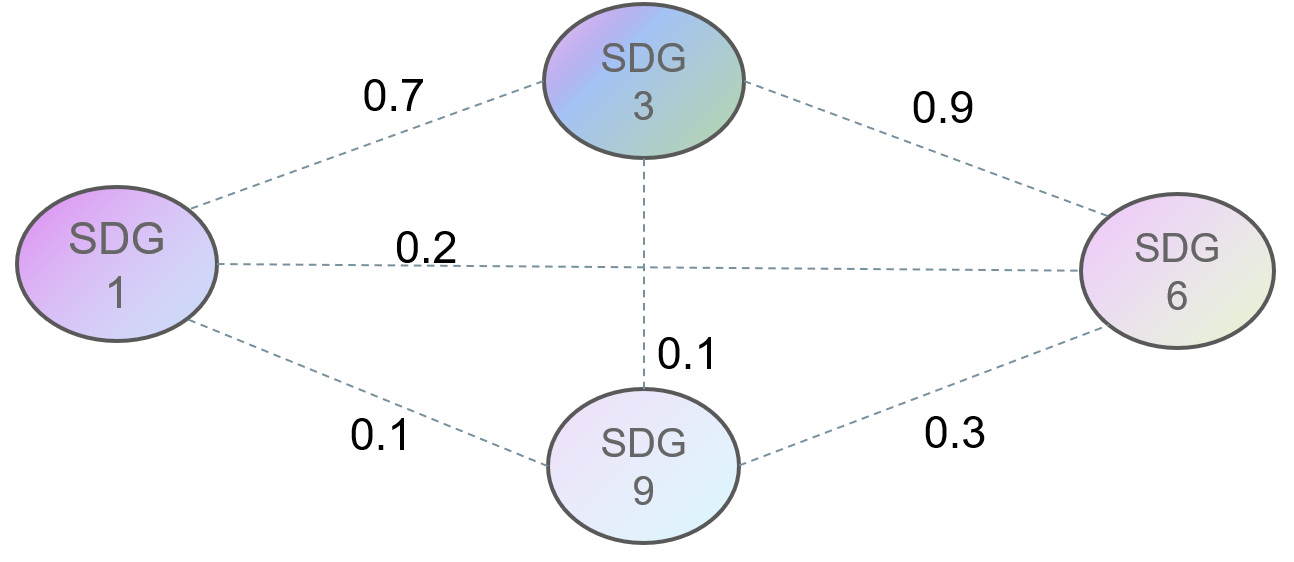
\includegraphics[width=7.0cm]{figures/example_v1.png}
        % \caption{ Raw Matrix}
        % \centerline{Raw Matrix}
    }
    \subfloat[]{
        \label{pic2}
        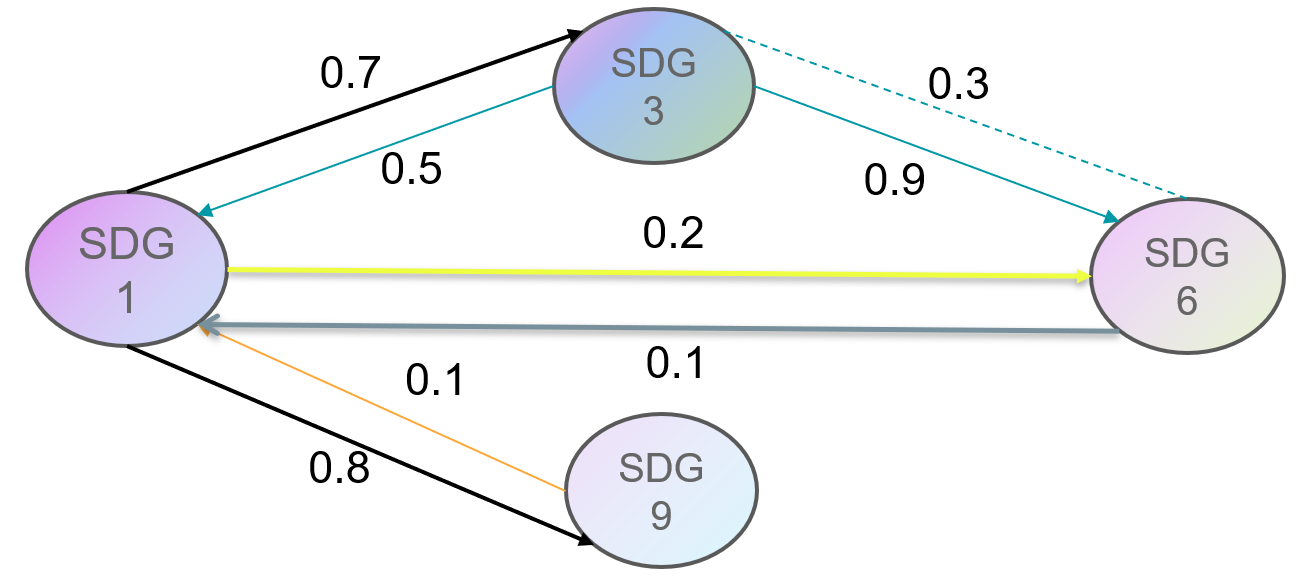
\includegraphics[width=7.0cm]{figures/example_v2.2.png}
        % \caption{After using the threshold }
        % \centerline{After using the threshold }
    }
    \caption{ An example of evaluation method  }%修一下,不能两行
    \label{fig.example}
\end{figure}



\subsection{Analysis of Experimental Results and Answers for Questions}%每个小节回答一个问题

The algorithms presented in this paper were implemented using Python 3.8 programming language and were run on a computer with an Intel Core i5-8250U @ 3.4GHz CPU and 8GB RAM. The simulation experiments were conducted in the following aspects:

\subsubsection{ Requirement 2: Analysis of reasonable achievement in 10 years}
\subsubsubsection{ Priorities that  efficiently move the work }


Using the network and specific SDGs to prioritize actions can enhance UN work successfully. Considering the assessment of the effectiveness of each priority and determining ten-year deliverables, the difficulty of finding priorities is translated into a sequential problem of traversing the
network structure.


Figure \ref{fig.gantt no over}  shows the priorities that will most effectively drive the work of the UN forward. The final solution of the multi-objective optimization model is the development priority order of the SDGs. We not only find the optimal priorities but also evaluate the priorities of each SDGs.

\subsubsubsection{Confidence level}

 It was found that most of the sustainable development goals do not follow a normal distribution. And the confidence level of the model results depends on the confidence level of the linkage matrix and how well the model fits the existing data. Therefore, we conducted two tests to make the data more reliable.

% Due to the fact that genetic algorithms are not probabilistic correlation models, the inference conclusions that genetic algorithms provide for a set of data are always deterministic.
It is necessary to begin with the correlation of the nodes in order to achieve an accurate representation of the model. As the binary adjacency matrix(see Table \ref{fig.prob}) that is used by the method is created by sampling the correlation matrix, the level of confidence that can be placed in the algorithm may be described in terms of the level of confidence that can be placed in the connection weights. 


\begin{figure}[H]
    \centering
    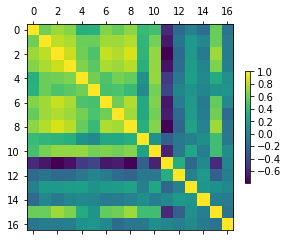
\includegraphics[width=5.5cm]{figures/prob.png}
    \caption{ Probability map of edges }%后面加注释
    \label{fig.prob}
\end{figure} 

We used time series data on the specific benefits and progress of each sustainable development goal as a basis. Then, we used linear regression to simulate the relationship between the progress of each sustainable development goal and its specific benefits, while controlling for any relevant factors. Finally, we compared the regression analysis results of each sustainable development goal. We used this information to calculate the target score for each sustainable development goal and to derive the final score for the overall effectiveness of the United Nations’ work. 
The MOEA/D algorithm adopts a dynamic weight allocation mechanism and local search operator to improve the convergence of the algorithm.

Finally, we take the arithmetic mean of the above two confidence levels and obtain a confidence level of 0.832 for the algorithm results. The results obtained by the MOEA/D algorithm are more robust and can handle a variety of complex multi-objective optimization problems, including those with non-convex, discontinuous, and multi-modal characteristics. 



\subsubsubsection{Reasonable to achieve in 10 years}



According to the data on the impact of different SDG priorities on investment costs and implementation times, the MOEA/D model was applied to process the data to get the non-dominated solutions. The Pareto front in the objective space according to these non-dominated solutions is shown in Figure \ref{fig.gantt no over}(a). Then we choose the knee point from these solutions (shown by a blue circle) as the final solution, and the Gantt Map according to this solution (priority sequence of the 17 SDGs) is shown in Figure \ref{fig.gantt no over}(b). From this figure, it can be seen that all of the SDGs can be finished within 14.23 years based on our assumption of the execution time of each SDG, and only 6 SDGs would not be handled within 10 years. In conclusion, all goals except SDG3, SDG16, SDG12, SDG9, SDG15 and SDG1 can be achieved in the next 10 years assuming that the execution of these SDGs does not overlap with each other.

\begin{figure}[h]
    \centering
    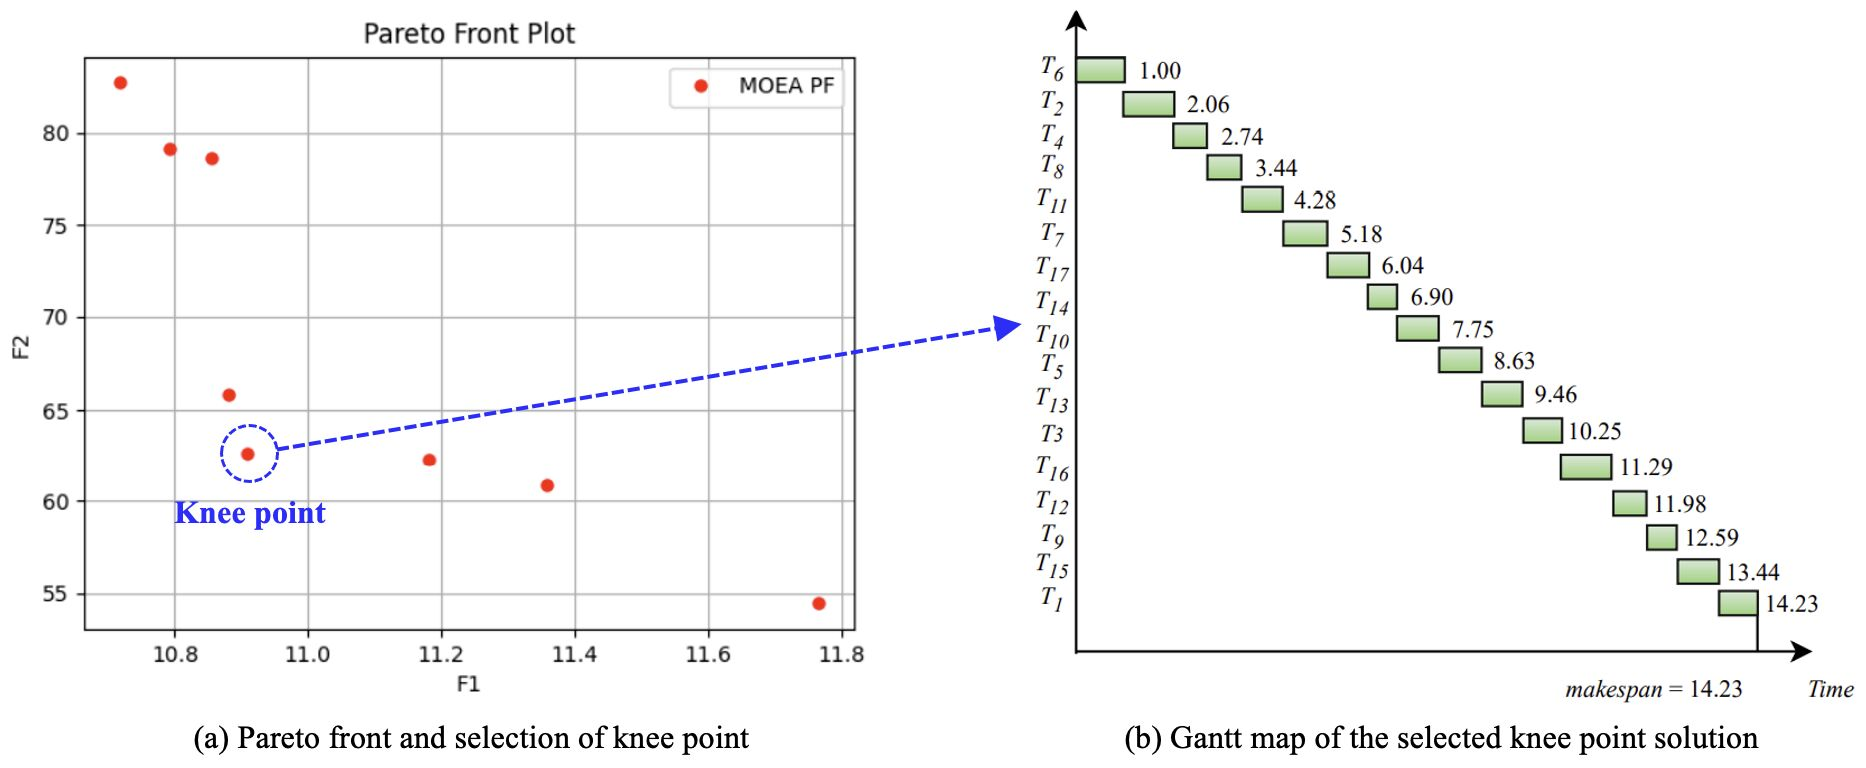
\includegraphics[width=16cm]{figures/Illustration.jpg}
    \caption{Illustration of Pareto front and Gantt map of selected knee point  }%后面加注释
    \label{fig.gantt no over}
    \vspace{-15pt}
\end{figure} 

\subsubsection{Requirement 3: Analysis of completion of a certain SDG}
% 如果实现了其中一项可持续发展目标(例如,没有贫困或没有饥饿),由此产生的网络结构将是什么?这一成就将如何影响您团队的优先事项?

Analyze the effects of reaching specific SDGs, such as eradicating poverty and hunger, on the network's structure and team priorities.
If one of the sustainable development goals is achieved, such as No Poverty, it will have a positive impact on other goals. This is because there are interdependent relationships among the sustainable development goals, and each goal interacts with and influences others. For example, if poverty is eradicated, more people will have access to education and healthcare, thus positively impacting the goals of 'Quality Education' and 'Good Health and Well-being'. Similarly, by achieving the goal of 'Zero Hunger', it can help improve the nutritional status of women and girls, contributing to the achievement of the goal of 'Gender Equality'.

% \noindent \textbf {(1) }
\subsubsubsection{If one SDG is achieved, what would be the structure of the resulting network?}

Using 'No Poverty' as an example of a completed goal: poverty is a primary obstacle to achieving all sustainable development goals. If we can eradicate poverty, it would be easier to achieve other sustainable development goals. In addition, eradicating poverty can also help reduce social instability and inequality.
Assuming that SDG 1 has been achieved, we constructed a new network of SDGs by using the method of requirement 1.

\begin{figure}[h]
    \centering
    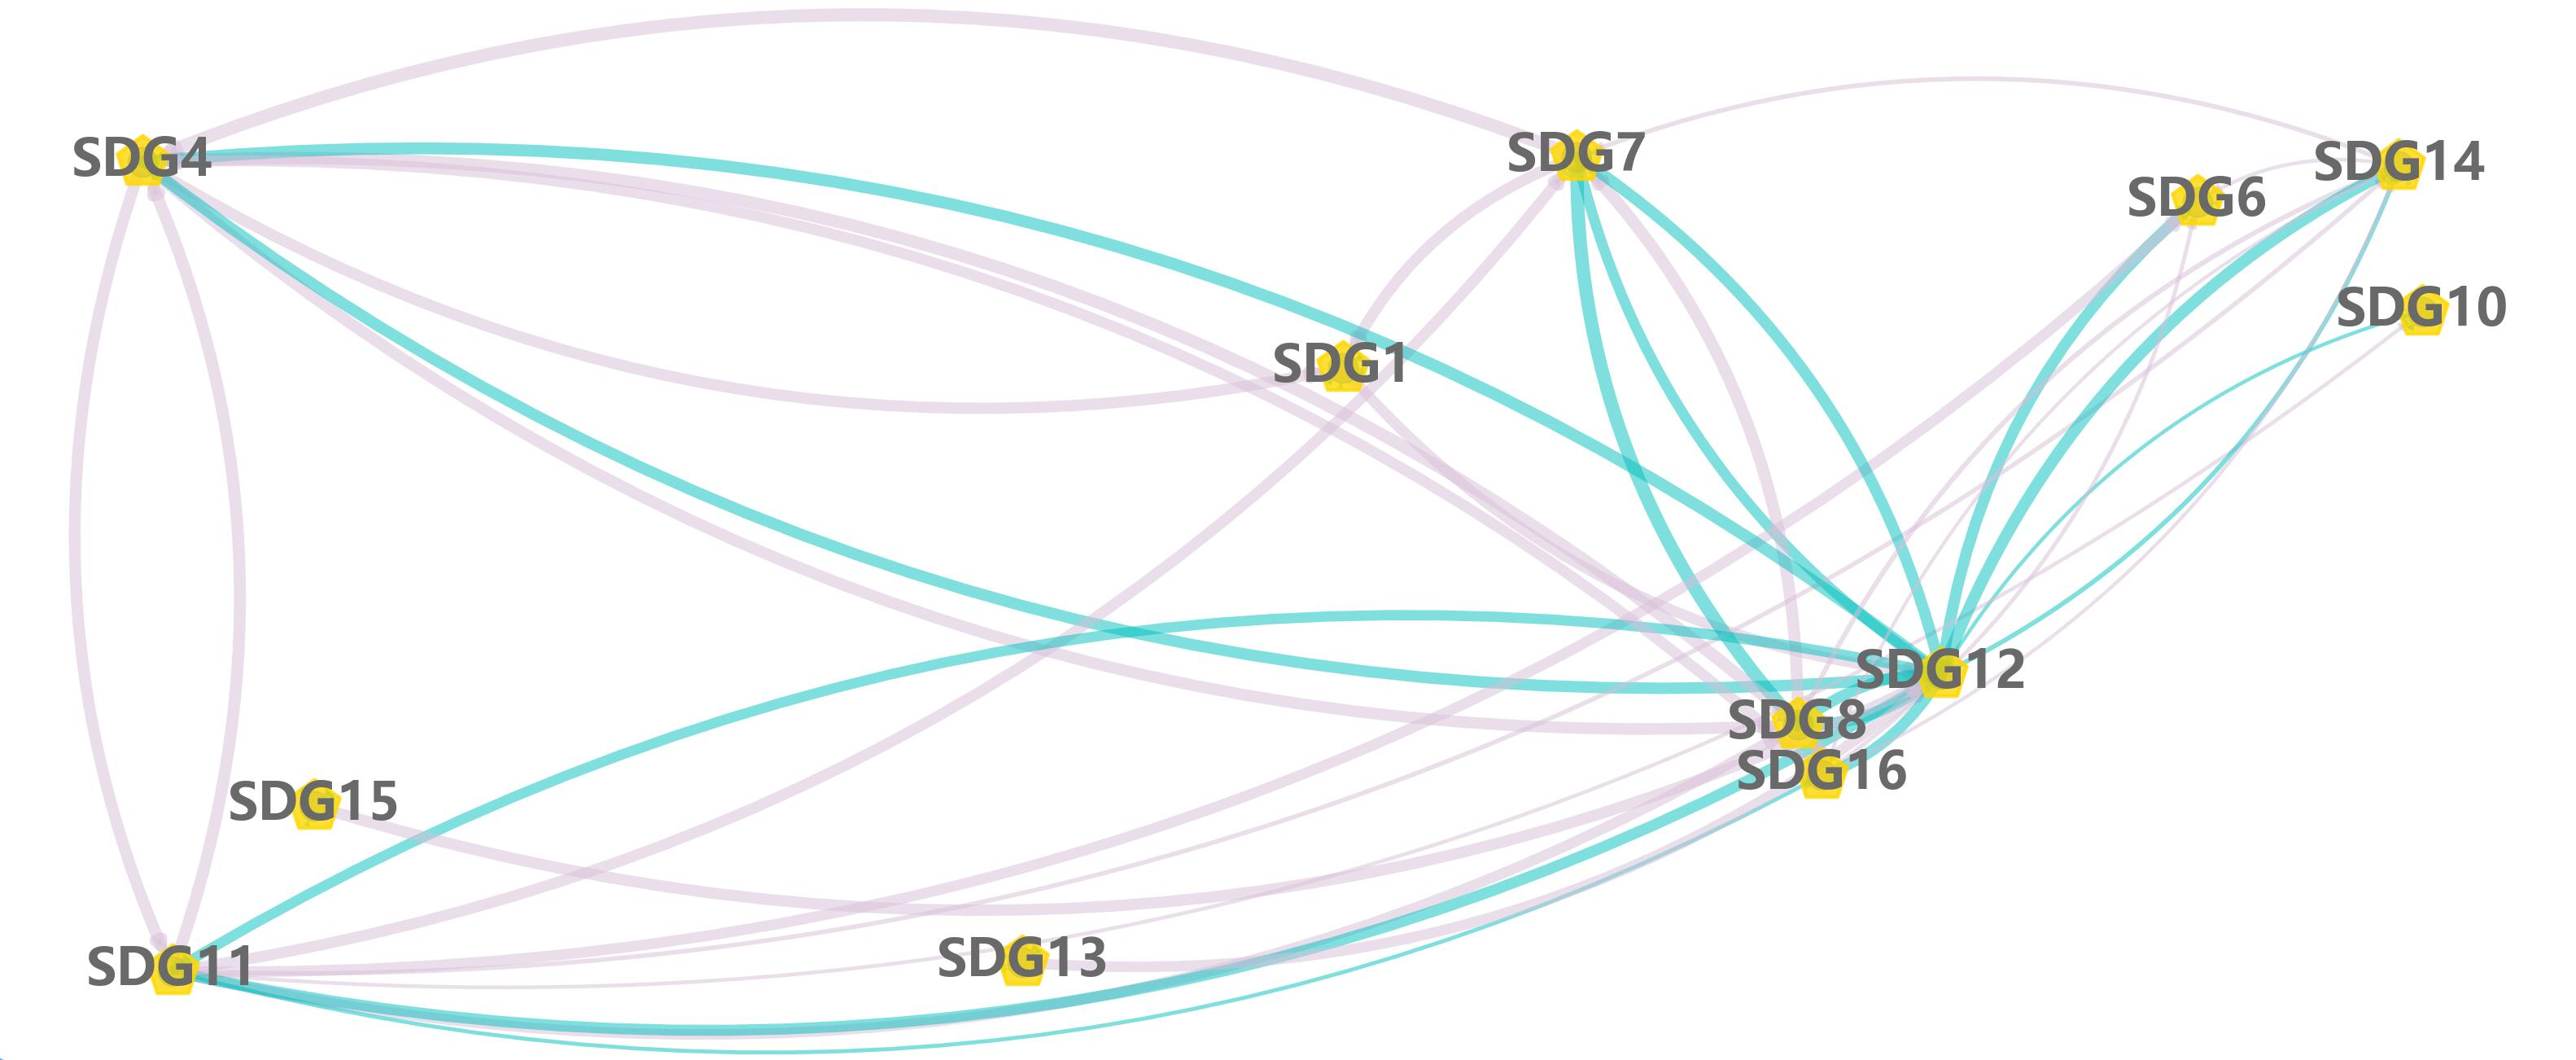
\includegraphics[width=9cm]{figures/Go to nodes.jpg}
    \caption{New Network of SDGs}%后面加注释
    \label{fig.new network}
    \vspace{-15pt}
    \small
\end{figure} 

Its implementation will have a positive impact on other sustainable development goals, thus helping to drive the entire sustainable development agenda. At the same time, its implementation will also enhance the interconnectivity of various nodes in the network, leading to significant progress in the overall sustainable development agenda.

After removing a node, we calculated the time required to complete all projects. Comparing Figure \ref{fig.new network} with Figure \ref{fig.graph}, it was found that prioritizing SDG4 over completing all other SDGs individually could shorten the time required to complete all projects and reduce costs.
Meanwhile, some correlation coefficients between two SDGs has be changed from navigate to positive such as SDG 14 and SDG 6.

Therefore, we conclude that selecting sustainable development projects that are suitable for a country's situation and economic conditions is a feasible and economical approach.
\subsubsubsection{How would this achievement impact your team’s priorities?}

Assuming SDG 4 can be achieved, the SDG indicators were re-analysed for correlation coefficients and an adjacency matrix was created.We used the MOEA/D algorithm for prioritisation of SDGs to obtain $S_1=(10,6,0,5,16,...,15)$ (the order of SDGs).Compared with the original order $S_0=(6,2,4,8,11,...,1)$,it is shown that the priority of SDGs have huge change if achieving one of goals.None of goals are the same to be possible to be achieved.

Regarding how this achievement will impact our team's priorities. If the goal of 'No Poverty' has already been achieved, we would choose 'Quality Education' as the next priority to achieve. On the one hand, quality education can help improve people's skills and knowledge, creating better job opportunities and higher income levels for them, which will help consolidate and strengthen the achievements made in eliminating poverty. On the other hand, quality education is also the foundation of other sustainable development goals, as only those who have received a good education can better understand, adapt to, and participate in the sustainable development process. For example, only those who have been educated can better achieve the 'Good Health and Well-being' goal and participate in the 'Gender Equality' and 'Peace and Justice Strong Institutions' goals.

Therefore, the two goals of 'No Poverty' and 'Quality Education' are related, and the order in which they are achieved has an important impact on the entire sustainable development process.


\subsubsubsection{Are there other goals that should be included or proposed to the UN for inclusion?}
\indent Introduce additional objectives for the network. We transform this problem into an analysis of the change in the knee points after the transformation of the model parameters. Through the analysis of the change in the knee points, we conclude that although the United Nations' sustainable development goals are comprehensive and detailed, specific challenges and issues may be encountered in the actual implementation process. Therefore, it may be necessary to propose some targeted supplementary or further refined goals. The followings are some areas or issues that may need to be included in the United Nations' sustainable development goals:

'Digitalization': With the rapid development and application of digital technology, digitalization has become an important area of social transformation. To ensure the sustainability of digitalization, some goals related to digital privacy, data security, digital equality, etc., can be added to the United Nations' sustainable development goals.

'Biodiversity': The maintenance and protection of biodiversity are crucial for the balance and sustainability of ecosystems. Therefore, some goals related to biodiversity conservation, such as protecting natural ecosystems, reducing species extinction, and restoring ecosystems, can be added to the United Nations' sustainable development goals.

'Citizen Responsibility and Participation': Citizen responsibility and participation are important prerequisites for achieving sustainable development. Therefore, some goals related to civic responsibility and participation, such as encouraging citizens to participate in social affairs and increasing citizens' sense of social responsibility, can be added to the United Nations' sustainable development goals.

These goals are closely related to sustainable development. If the United Nations can further emphasize these issues in the future sustainable development agenda, it will help promote the process of sustainable development more effectively.

% 通过利用多目标优化算法,我们找到了最适合的候选者应具备的品质。它应对已有SDGs有如下相关性,来保证其对现有优化顺序的提升。
By using a multi-objective optimization algorithm, we find the qualities that the most suitable candidate should have. It should have the following relevance to the existing SDGs(see Table \ref{tab. pre weights of SDG}) to ensure its enhancement to the existing optimization order. 

\begin{table}[h]\caption{ Predicted Weights of the SDGs }
\centering
\label{tab. pre weights of SDG}
\tiny
\tabcolsep=0.1cm
\begin{tabular}{lccccccccccccccccc}
\hline
\multicolumn{1}{c}{} & SDG1  & SDG2  & SDG3  & SDG4  & SDG5  & SDG6  & SDG7  & SDG8  & SDG9  & SDG10 & SDG11 & SDG12 & SDG13 & SDG14 & SDG15 & SDG16 & SDG17 \\ \hline
Raw                  & 0.111 & 0.039 & 0.039 & 0.005 & 0.022 & 0.012 & 0.029 & 0.042 & 0.045 & 0.075 & 0.038 & 0.198 & 0.098 & 0.075 & 0.070 & 0.001 & 0.102 
\\ \hline
\end{tabular}
\end{table}

% 是否还有其他目标应该包括或建议联合国纳入?

\subsubsection{Requirement 4: Analysis of influential factors such as technological advances}
% 	从网络的角度来看,对联合国的进展有哪些重大影响?
% 		灵敏度分析
% 			技术进步对其他的影响,导致时间发生变化
% 		比较前后变化,看影响
% 		节点权重参数fine-tune
% 			导致优先级变化
% 			进而给出建议
\subsubsubsection{Discuss the impact of technological advances, global pandemics, climate change, regional wars, refugee movements, or other international crises on your team’s network and your team’s choice of priorities.}


 Climate change\cite{conway2010united}, global environmental governance\cite{kumar2020united}, humanitarian crisis\cite{omgba25topic} or other international crises are having a positive or negative impact on the progress of the United Nations. Considering this international crisis will have an impact on some SDG indexes such as the influence of climate change on SDG 13(Climate Action), there follows a change of weights of SDGs. Here is an example of technological advances.
 % 这里以  technological advances 为例子。

 % 对于我们的模型,网络参数
 So we set an  impact factor to adjust some weights of SDGs by using AHP, then calculated the Spearman rank correlation coefficient of SDGs which can be drawn adjacency matrix. Finally, a relevance network between SDGs was constructed. These values in Table \ref{tab.weights of SDG}  are generated by the AHP algorithm. 

\begin{table}[h]\caption{ Weights of the SDGs }
\centering
\label{tab.weights of SDG}
\tiny
\tabcolsep=0.1cm
\begin{tabular}{lccccccccccccccccc}
\hline
\multicolumn{1}{c}{} & SDG1  & SDG2  & SDG3  & SDG4  & SDG5  & SDG6  & SDG7  & SDG8  & SDG9  & SDG10 & SDG11 & SDG12 & SDG13 & SDG14 & SDG15 & SDG16 & SDG17 \\ \hline
Raw                  & 0.011 & 0.039 & 0.033 & 0.011 & 0.032 & 0.002 & 0.009 & 0.042 & 0.045 & 0.035 & 0.038 & 0.198 & 0.198 & 0.115 & 0.070 & 0.001 & 0.122 \\
Changed              & 0.013 & 0.041 & 0.033 & 0.011 & 0.032 & 0.005 & 0.009 & 0.042 & 0.045 & 0.035 & 0.038 & 0.194 & 0.198 & 0.115 & 0.040 & 0.000 & 0.122 \\ \hline
\end{tabular}
\end{table}

 In addition, huge changes in the environment not only affect the size of weight values of SDGs, but also have an impact on the network structure. For example, when an SDG has a score of more than 100−e100-e, we consider that the task has been reached. The amount of its contribution to other nodes will be retained,  but itself will be removed from the graph.
 
 % 网络图
 \begin{figure}[h]
    \centering
    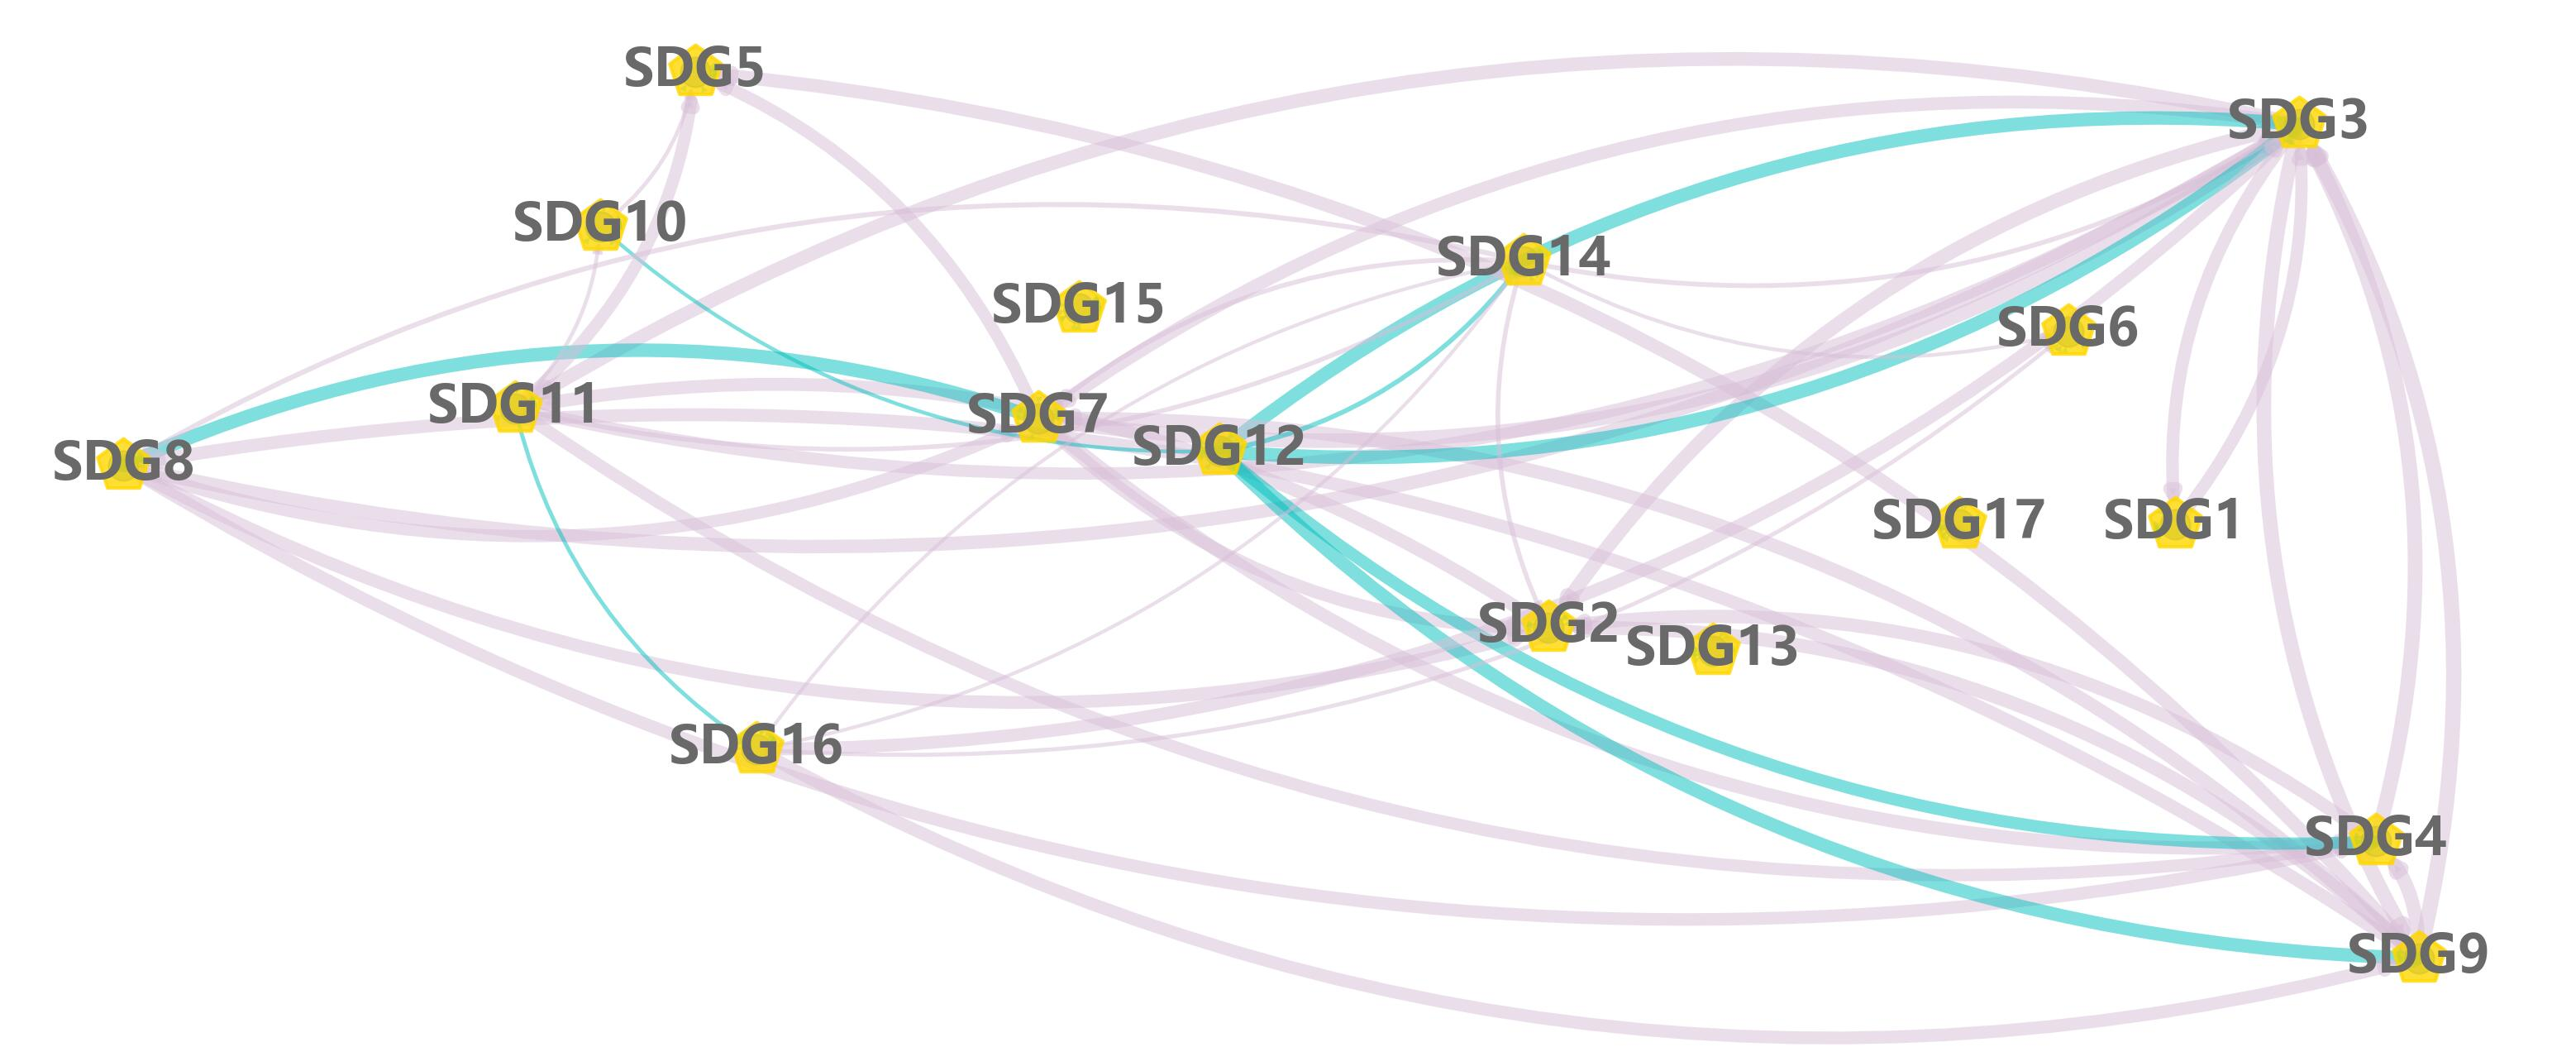
\includegraphics[width=8cm]{figures/graph.jpg}    
    \caption{ Modified network of SDGs}%后面加注释
    \label{New Network Of SDGs }
\end{figure} 

Then We applied the MOEA/D model to impact prioritisation on investment costs and implementation time matrix. We can see clearly that order of the achievement of 17 goals has changed from Figure \ref{Pareto Front} below.

% 使用新的权重和网络后,模型的knee点出现了明显的不同。 
After using the new weights and network, the knee points of the model appear significantly different(see Figure \ref{knee_compare}).  According to the knee point selection formula($\max (W_1*f_1 + W_2*f_2 )$), we find that such an environmental change can make a decisive contribution to the knee point selection.
% knee点计算
% 比如两个目标f1 f2; 选择knee点的方式就是计算0.5*f1+0.5*f2, 对接进行排序,最大值得那个就是
 \begin{figure}[H]
    \centering
    \subfloat[]{
        \label{picww}
        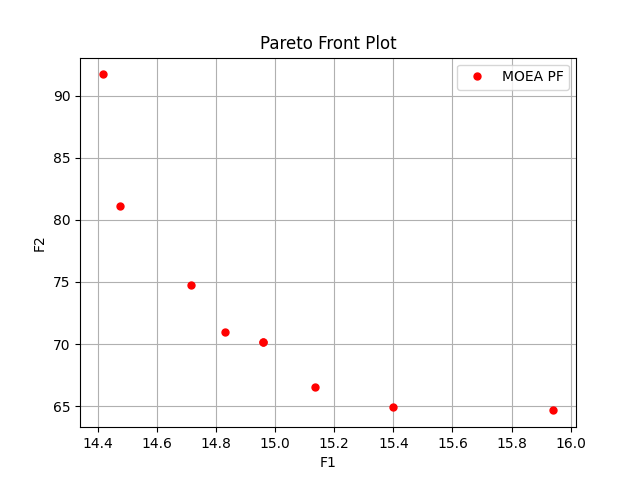
\includegraphics[width=5.0cm]{figures/decrease_no_over.png}
        % \caption{After using the threshold }
        % \centerline{After using the threshold }
    }
    \subfloat[]{
        \label{picee}
        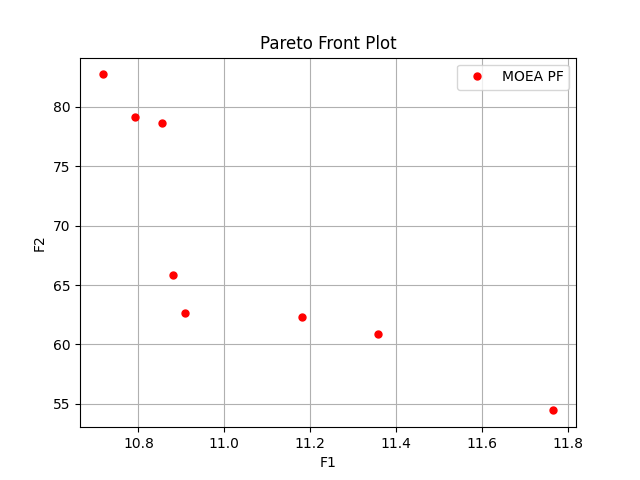
\includegraphics[width=5.0cm]{figures/No_overlap.png}
        % \caption{After using the threshold }
        % \centerline{After using the threshold }
    }
    
    \caption{ Comparison of knee points based on the impact of influential factors  }%修一下,不能两行
    \label{knee_compare}
\end{figure}

% a、b展示了变化前后搜索到的顺序。通过两张图片的对比可以看出,加入overlap后模型的makespan明显减少。

% 图
 

% \begin{figure}[h]
%     \centering
%     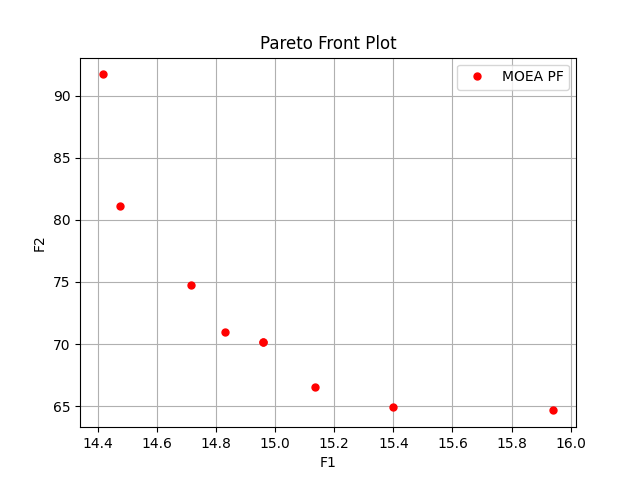
\includegraphics[width=6.5cm]{figures/Figure_1.png}
%     \caption{ Pareto Front}%后面加注释
%     \label{Pareto Front }
% \end{figure} 
% % \vspace{-15pt}


\subsubsubsection{What is the major impact on the progress of the UN from a network perspective?}
\indent It is shown that SDG 6 ranks first followed by SDG 1, SDG 7, SDG 8 and SDG 5. This means SDG 6 is the most likely to be achieved in ten years due to the least possible time and cost. Compared with requirement 2, only SDG 7 is more likely to be achieved as the same as it. So did these factors impact the UN's network-based progress from Figure\ref{Pareto Front}.
\begin{figure}[H]
    \centering
    
    \subfloat[]{
        \label{picq}
        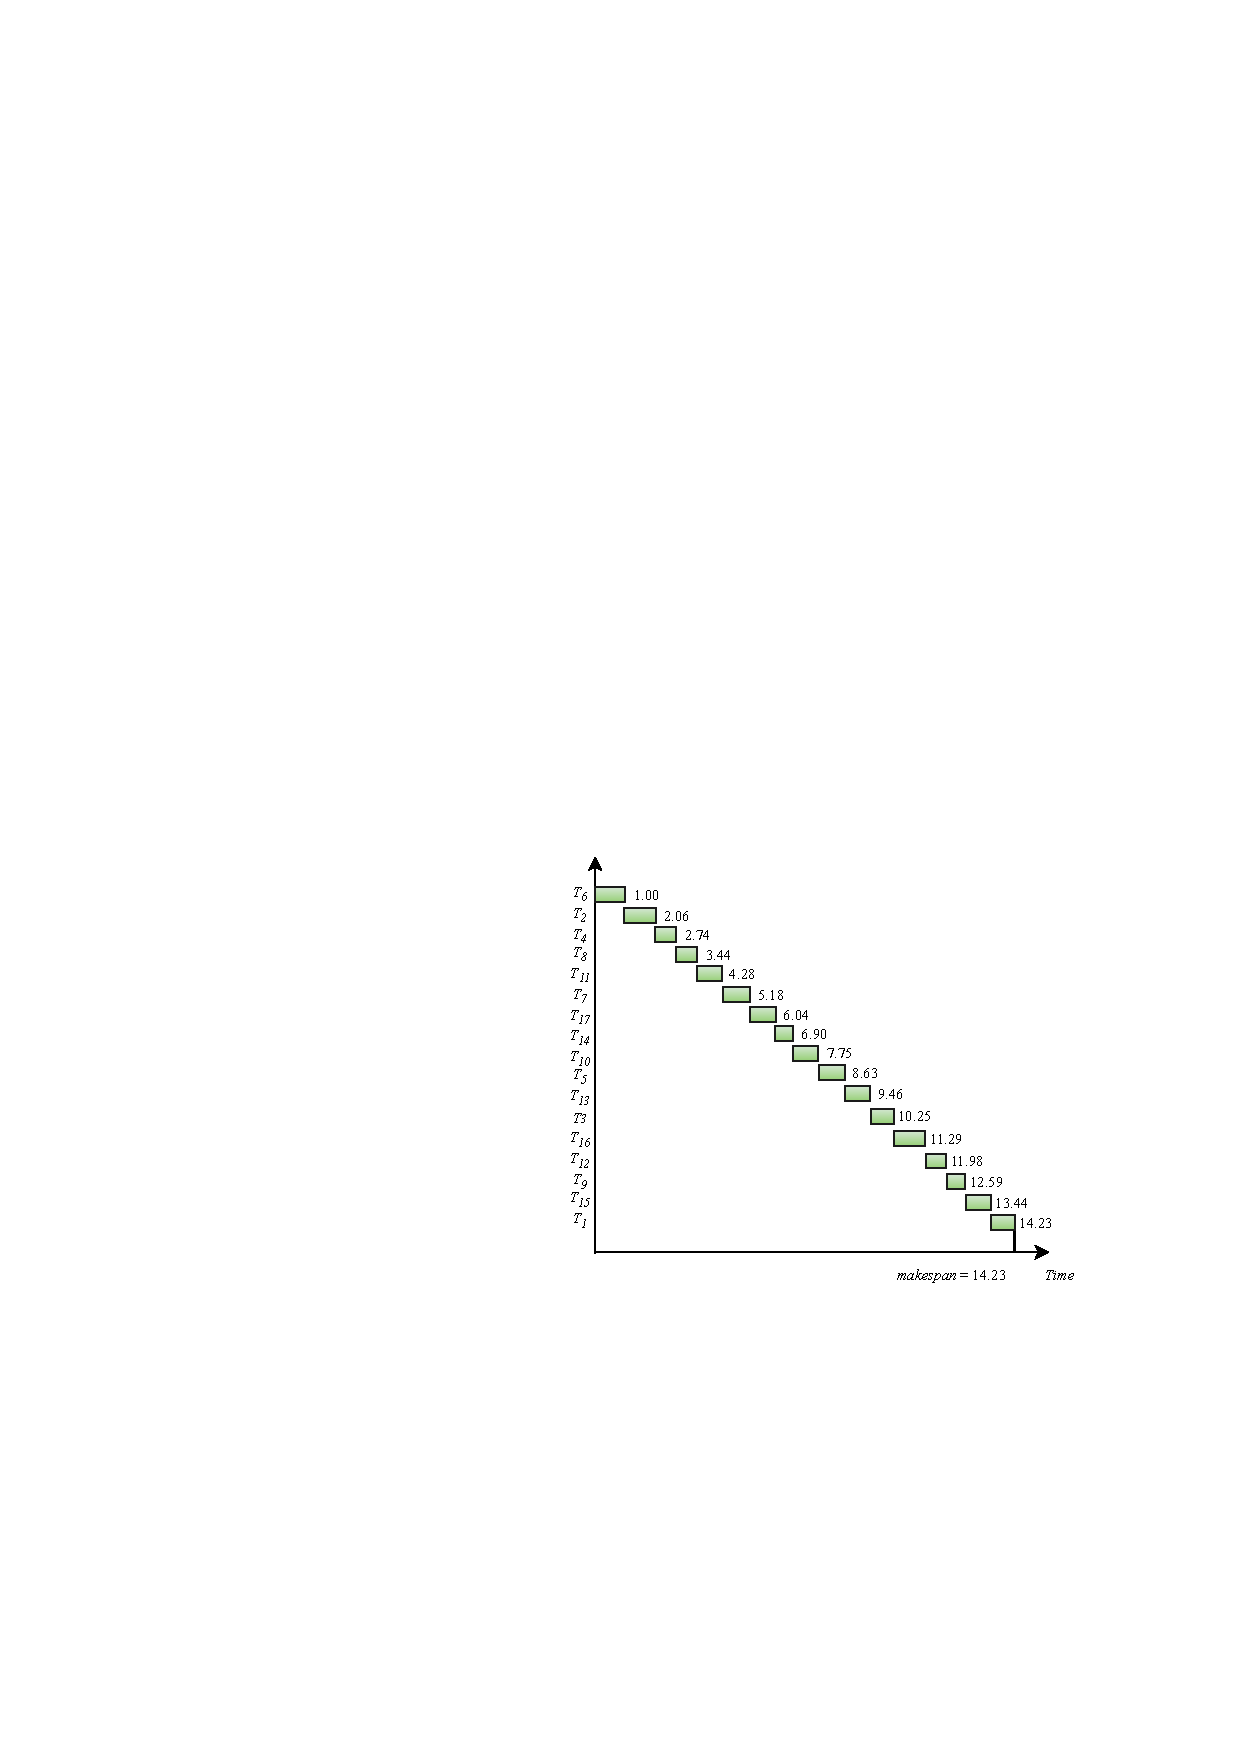
\includegraphics[width=5.0cm]{figures/Nooverlap-Gantt.pdf}
        % \caption{ Raw Matrix}
        % \centerline{Raw Matrix}
    }
    \subfloat[]{
        \label{picw}
        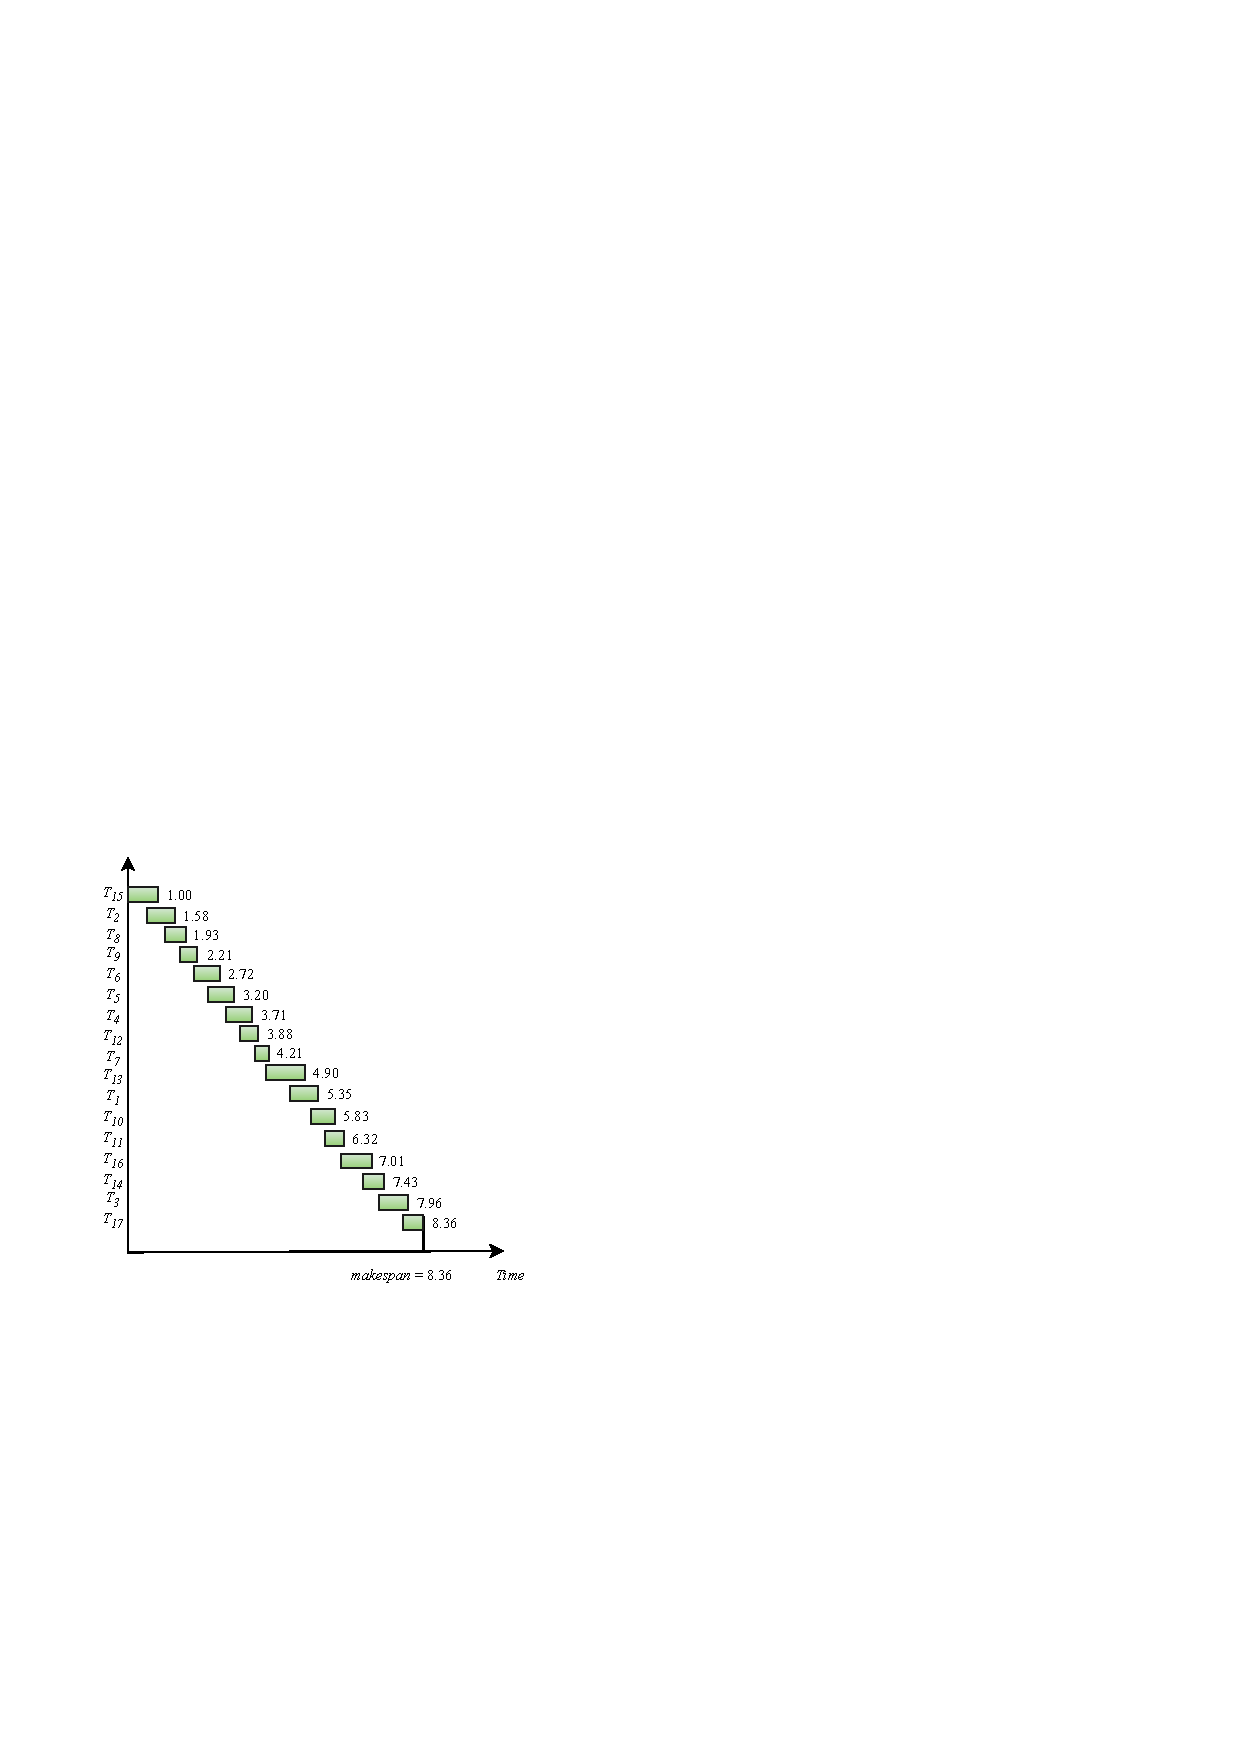
\includegraphics[width=4.5cm]{figures/Overlap-Gantt.pdf}
        % \caption{After using the threshold }
        % \centerline{After using the threshold }
    }
    % \subfloat[]{
    %     \label{pice}
    %     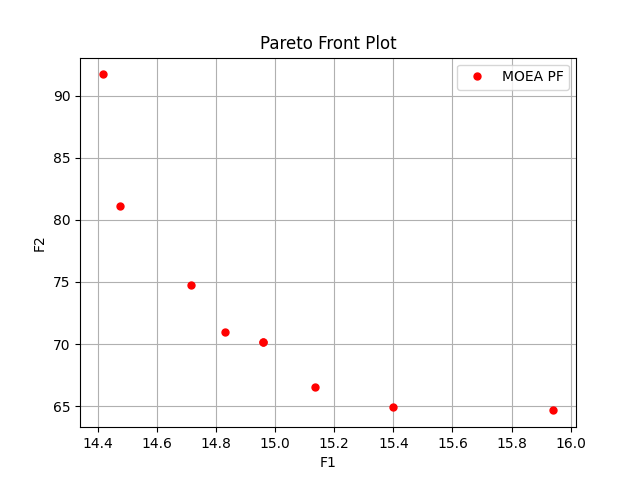
\includegraphics[width=5.0cm]{figures/Figure_1.png}
    %     % \caption{After using the threshold }
    %     % \centerline{After using the threshold }
    % }
    
    \caption{ Comparison of priority sequences based on the impact of influential factors  }%修一下,不能两行
    \label{Pareto Front}
\end{figure}

$\bullet$ Technological advances: 
The impact of technological advances on the UN has been twofold. On the one hand, new technologies have given the UN more tools and means to respond to disasters, crises and humanitarian assistance, while also increasing its efficiency and responsiveness. On the other hand, advances in technology have also brought new challenges and threats, such as cyber security issues and threats in virtual spaces.

$\bullet$ Global pandemics: 

Global pandemics have a significant impact on the UN as they can lead to global health emergencies that require a  response from the UN  to provide health assistance and coordinate global efforts to combat epidemics.

$\bullet$ Climate change: 

Climate change has far-reaching global environmental, economic and social impacts, which need UN environmental agencies such as the United Nations Environment Programme to work to address climate change, coordinate national action to reduce emissions and promote global sustainable development.

$\bullet$ Regional wars:

Regional wars can lead to the displacement of millions of people and create humanitarian crises. UN peacekeeping operations work to maintain international peace and security, mediate conflicts, protect civilians and provide humanitarian assistance.

$\bullet$ Refugee movements: 

Refugee movements are a global problem, with implications for UN agencies and governments. Agencies such as UNHCR and the International Organisation for Migration (IOM) provide refugee protection and relief services and coordinate with governments on refugee admission and resettlement
% 相当于网络结构变化后,knee点 !!!!!!!!!!!!!!!!!!!!!!!!!!!!!!
% 最小费用最大流
% 政策、疫情等影响转变为权重值、网络参数变化下的多目标优化问题。





\section{Case \uppercase\expandafter{\romannumeral2} : Modeling with overlap between two SDGs }
% 不能写中文,得用百分号注释



\subsection{Model Characteristics}%介绍一下这一节考虑的情况:如果允许相邻的两个SDG可以overlap
In order to improve the model's applicability in the real world, we will make the following assumption over the course of this chapter: It is acceptable for two neighbouring SDGs to overlap with one another. This indicates that the execution of the subsequent Tasks can begin even though the prior task has not yet been completed.

\subsection{Mathematical Model}
% \subsubsection{}
Since only minor changes were made to the model, we retained the parameter variables as in Table 6 and the decision variables as in Table 7. Since the optimization objective of the model remains unchanged, the objective function of the model is unchanged.


The start time of SDG $\pi_{i}$ is equal to the completion time of the previous SDG $\pi_{i-1}$ minus the overlap time $q_i$ of SDG $\pi_{i}$
\begin{equation}
s_{\pi(i)}=e_{\pi(i-1)}-q_i, \quad(i=2,3, \ldots, n)
\end{equation}

At the same time, up to two SDGs are allowed to be implemented.:
\begin{equation}
    e_{\pi(i)}  \leq  s_{\pi(i+2)}  \leq e_{\pi(i+1)},          (i,=1,2,...,n-2)
\end{equation}

\subsection{Decomposition-based multi-objective evolutionary algorithm (MOEA/D)}%简要介绍一下算法,因为与之前3.3节相同,因此只介绍变化的部分
Since the MOEA/D has been described in Section 3.3, in this section we only present the modification of it to adapt to the current model.

Figure \ref{fig.over} shows the combination of priorities that will most effectively drive the work of the United Nations. The final solution of the multi-objective optimization model is the development priority order of the SDGs. We not only identify the optimal priorities but also evaluate the priorities of each SDG. Additionally, Figure \ref{fig.over} also provides the lead time for each SDG, indicating how far in advance each sustainable development goal should be started.


\begin{figure}[H]
    \centering
    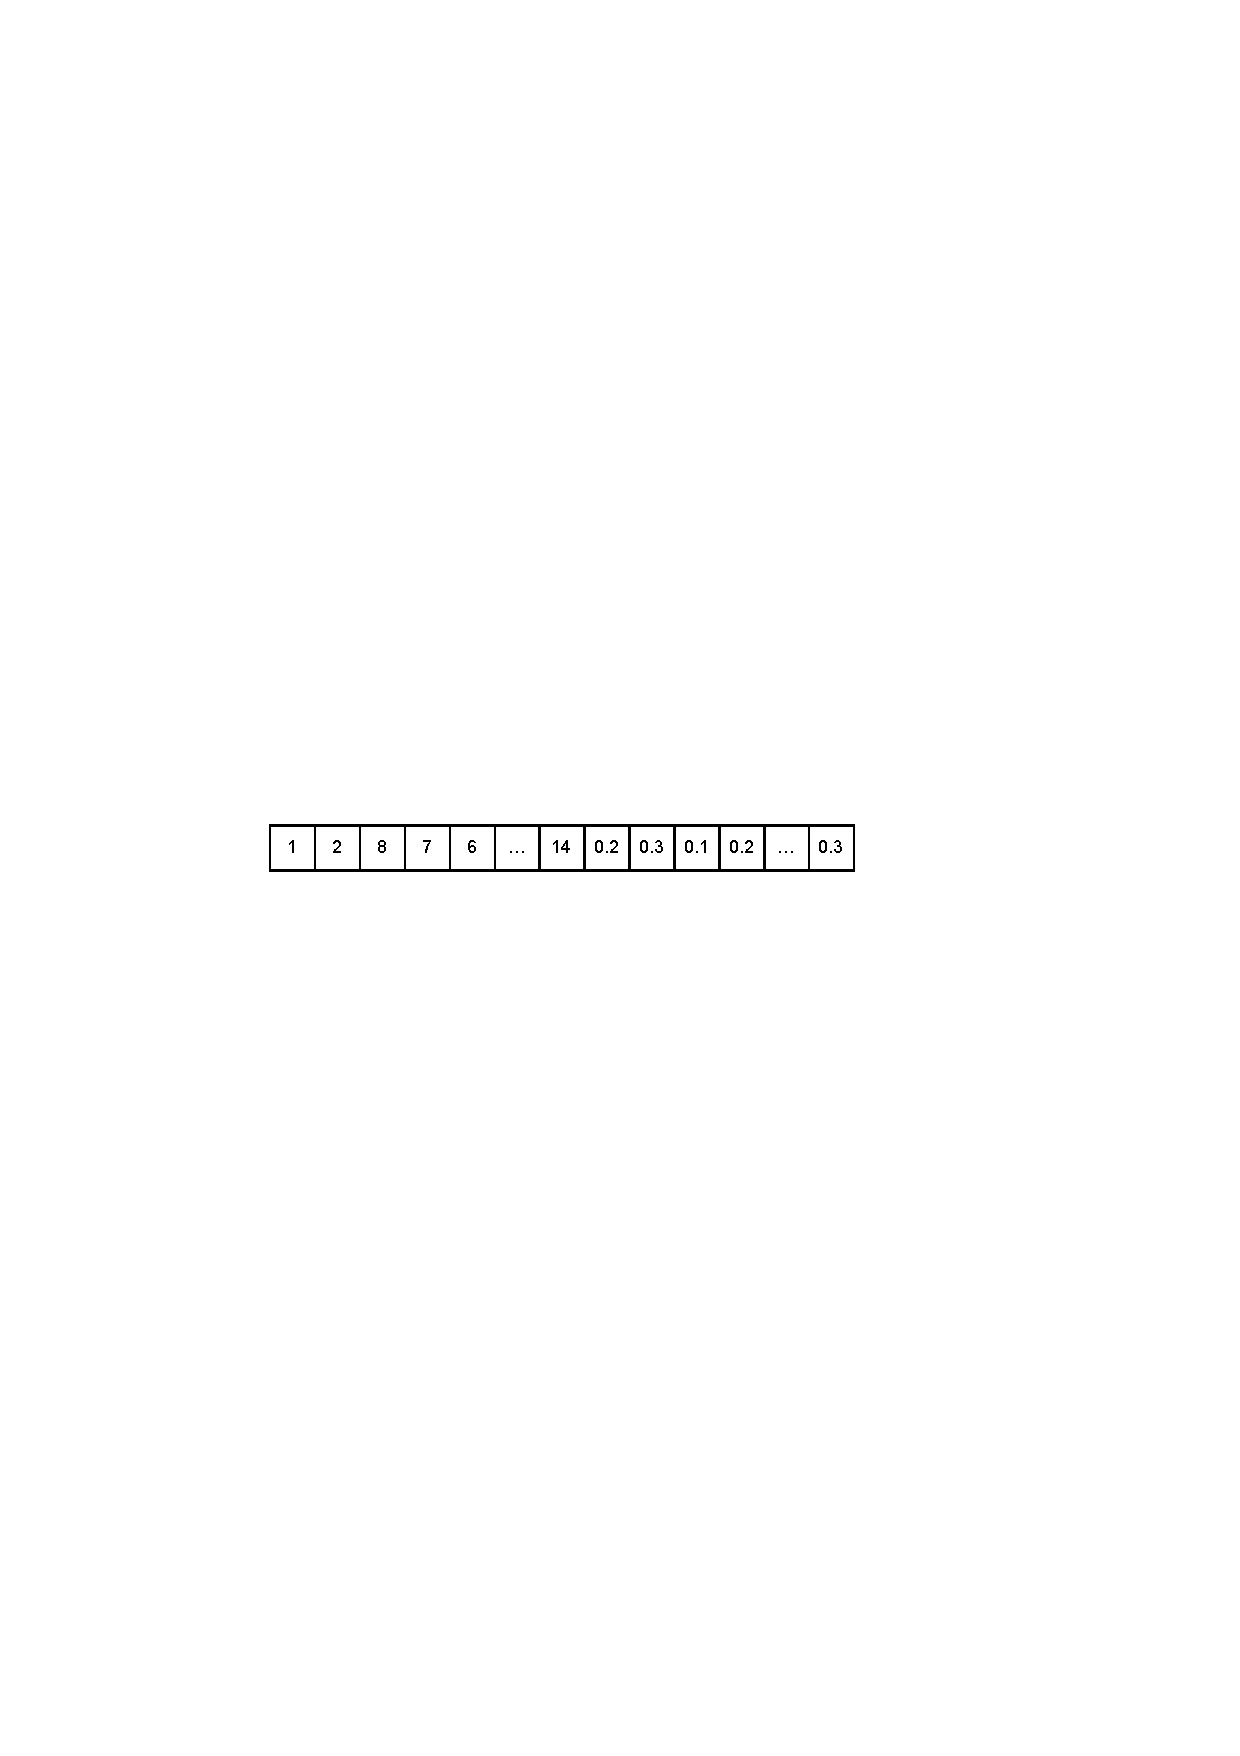
\includegraphics[width=10.0cm]{figures/Overlap figure.pdf}
    \caption{ Overlap }%后面加注释
    \label{fig.over}
\end{figure} 
\vspace{-15pt}

The decimal part in the table means how many years earlier each SDG should be started in the corresponding order.

\subsection{Analysis of Experimental Results and Answers for Questions}%每个小节回答一个问题
We kept most of the experimental settings from the previous section and only changed them in the overlap position.%在该模型中,我们设置了两个SDG可同时作为优先事项达成,并保留了其他所有设置。

\subsubsection{Requirement 2: Analysis of reasonable achievement in 10 years}


In the single-objective optimization model, the top five priority SDGs determined from the results, as shown in Figure \ref{fig.noover}, were SDG 1, SDG 2, SDG 6, SDG 4, and SDG 8. In the dual-objective optimization model presented in this chapter, the top five priority SDGs determined from the results, as shown in Figure \ref{fig.over}, were SDG 1, SDG 2, SDG 8, SDG 7, and SDG 6.

There were significant differences between the two models in the third to fifth priority SDGs, with the dual-objective model being more accurate in cases of ample funding.

In this chapter, we assumed that two SDG can overlap, meaning that two goals can be invested in at the same time. Based on data on the impact of different SDG priorities on investment costs and implementation times, we applied the MOEA/D model to process the data and obtain the minimum time and costs. A Gantt chart of 'With Overlap' was drawn to show the sequencing among the 17 sustainable development goals. Figure \ref{fig.gantt over} shows the results obtained from our model. All tasks will be completed within 8.36 years, which means that all 17 tasks can be completed in the next 10 years assuming that two sustainable development goals can overlap. In conclusion, all goals can be achieved in the next 10 years, and it will take only 8.36 years to complete the last task (SDG17).

\begin{figure}[H]
    \centering
    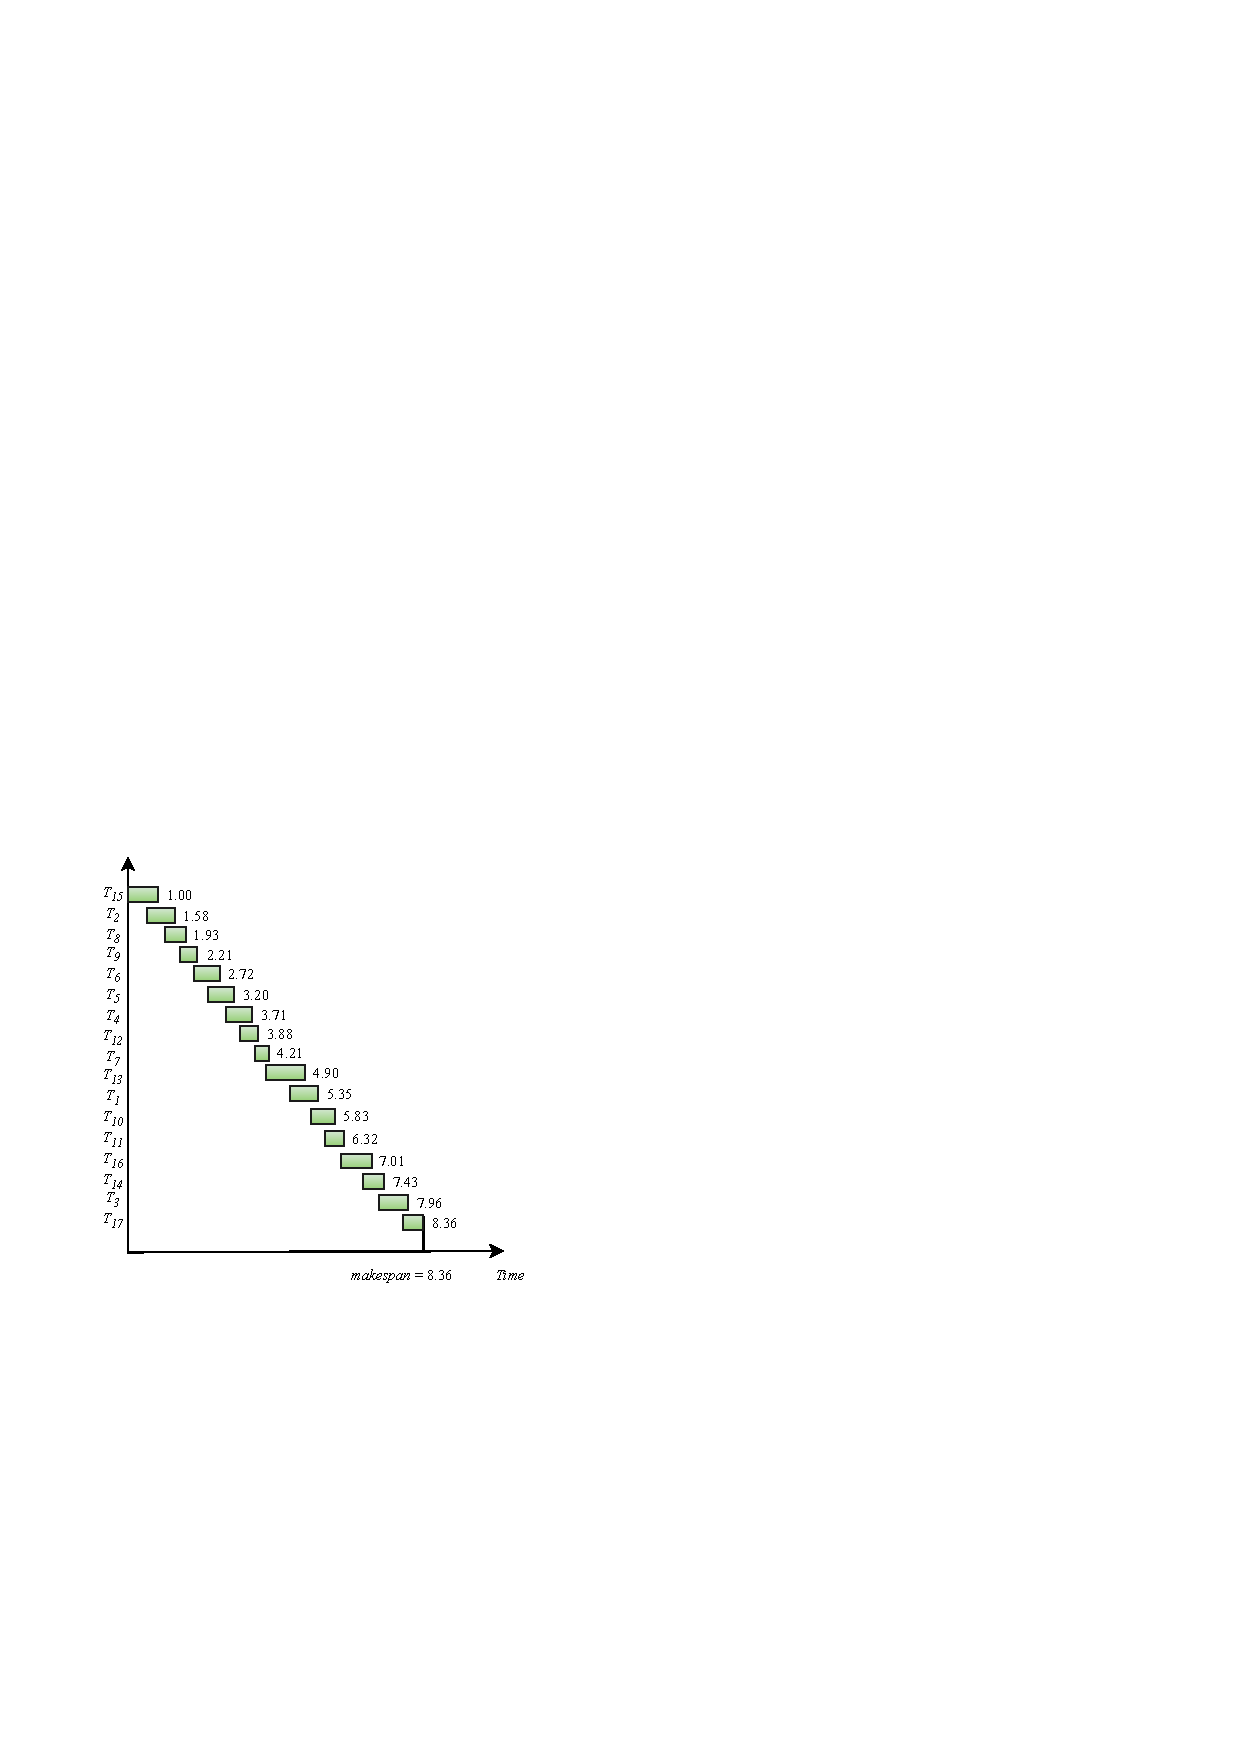
\includegraphics[width=6.0cm]{figures/Overlap-Gantt.pdf}
    \caption{ Gantt map of overlap case }%后面加注释
    \label{fig.gantt over}
\end{figure} 
\vspace{-15pt}

\subsubsection{Requirement 3: Analysis of completion of a certain SDG}
In this model, the network structure is relatively unchanged compared to the structure in section 3.3. However, since two sustainable development goals can be pursued simultaneously, there will be some promotion of synergies. Implementing two goals can promote synergy among different fields and stakeholders, such as combining poverty reduction and economic growth. This will strengthen the integrity of the sustainable development goals and achieve more long-term sustainable development.
At the same time, achieving two goals simultaneously can promote the coordinated use of resources and the environment. For example, reducing poverty and promoting sustainable energy at the same time will reduce the pressure on natural resources, thereby improving sustainability.

\subsubsection{Requirement 4}

When discussing the impact of factors such as technological advancement, global pandemics, climate change, regional conflicts, and refugee movements on the internet, there are several advantages to pursuing dual objectives simultaneously:

Facilitates more comprehensive discussions of issues. Achieving multiple goals simultaneously can promote synergies among different sectors and stakeholders, leading to more comprehensive discussions of the issues at hand. This can help advance the UN's work and progress across multiple fields.

Improves efficiency. Pursuing multiple goals simultaneously can improve efficiency, leading to the faster achievement of more goals. This is particularly important for addressing multiple international crises.

Promotes sustainability. Pursuing multiple goals simultaneously can promote the coordinated use of resources and the environment, leading to greater sustainability. This is particularly important for addressing issues such as climate change.

\section{Case III: Modeling with overlap between multiple SDGs }

In Case iI, we will study the last model in this article, the multi-objective overlapping model in scheduling problems. In the case of limited total resources, compared to the models in Case I and Case i, this model will give us the most optimal solution in terms of benefits.
Specifically, for this problem, it means that the United Nations can implement two or more SDGs at the same time, and in the case of ample funding, this model will provide the most efficient results. As the most complex model, it is also closest to a real-world situation.
%在Case iI中,我们将研究本文章中的最后一个模型,即调度问题中的多目标重叠模型。在资源总量有限的情况下,相比与Case I与Case i的模型,该种模型将能得出我们给出的效益最有解。
%具体化到本问题中,即意味着联合国可同时进行两项及更多项SDG的实现,在资金成本十分充裕的情况下,该模型将给出最优效率的结果。作为最复杂的模型,该模型也最接近现实中的情况。

\subsection{Model Characteristics}%介绍一下这一节考虑的情况:如果允许相邻的两个SDG可以overlap
In contrast to Case 1 and Case 2, the following assumptions will be made in the course of this chapter:the overlap of multiple SDGs is acceptable. This suggests that later tasks can be started even if the earlier ones have not yet been completed. At the same time, we expand the model to multiple overlapping goals than the overlapping of two adjacent SDGs in Case 2.
\subsection{Mathematical Model}
%在使用新模型的同时,我们保留了Case I与Case i中的参数、变量以及目标。并采用多目标重叠的新算法来构建模型。
Since only minor changes were made to the model, we retained the parameter variables as in Table 6 and the decision variables as in Table 7. Since the optimization objective of the model remains unchanged, the objective function of the model is unchanged.
Therefore, only one constraint is added to the Case I model.

The start time of SDG $\pi_{i}$ is equal to the completion time of the previous SDG $\pi_{i-1}$ minus the overlap time $q_i$ of SDG $\pi_{i}$
\begin{equation}
s_{\pi(i)}=e_{\pi(i-1)}-q_i, \quad(i=2,3, \ldots, n)
\end{equation}

\subsection{Decomposition-based multi-objective evolutionary algorithm (MOEA/D)}%简要介绍一下算法,因为与之前3.3节相同,因此只介绍变化的部分
The MOEA/D used for Case III is the same one as used for Case II, so the description of it is can be found in Section 4.3.

\subsection{Analysis of Experimental Results and Answers for Questions}%每个小节回答一个问题
We kept most of the experimental settings from the previous section and only changed them in the overlap position.%在该模型中,我们设置了两个SDG可同时作为优先事项达成,并保留了其他所有设置。

\subsubsection{Requirement 2: Analysis of reasonable achievement in 10 years}

In the experiment, the top five priority SDGs determined from the results are SDG1, SDG2, SDG8, SDG7, and SDG6. We analyzed the results and found that in the case of sufficient funding, the differences between the results obtained in Case III and Case I in selecting priority development goals are small. Therefore, the answer to this question is the same as in Case I, and we will not repeat it here.

\subsubsection{Requirement 3: Analysis of completion of a certain SDG}
In this model, compared to the structures in the previous two sections, the network structure has closer connections. Therefore, multiple goals can be achieved at the same time, allowing for more efficient use of resources and cost reduction. For example, the goals of 'Affordable and Clean Energy,' 'Climate Action,' and 'Clean Water and Sanitation' can be achieved in the same project, saving costs and improving efficiency in terms of time.

Moreover, sustainable development goals are interrelated and integrated, and achieving multiple goals simultaneously can better reflect this interconnection and integration.

\subsubsection{Requirement 4: Analysis of influential factors such as technological advances}

The impact of international crises such as technological advancements, pandemics, climate change, regional conflicts, and refugee movements on the network of relationships among the United Nations' 17 sustainable development goals is multifaceted. With the introduction of multi-objective optimization models, the relationship network becomes even more complex. Here are some of the key impacts and potential challenges that may arise:

Collaboration among goals: Events such as pandemics, climate change, regional conflicts, and refugee movements can affect the collaboration among the 17 sustainable development goals of the United Nations. For example, when faced with a large influx of refugees, the UN may need to simultaneously advance the goals of 'Reduced Inequality,' 'No Poverty,' and 'Good Health and Well-being' to help refugees integrate into local communities, reduce inequality, and improve their well-being.

Data collection and sharing: 'Industry, Innovation and Infrastructure' can promote data collection and sharing to help the UN better monitor and evaluate its progress towards sustainable development goals. However, in some cases, such as pandemics and wars, data collection and sharing may be affected, which may hinder the UN's assessment and monitoring of goal achievements.

Allocation of funding and resources: In the face of multiple crises, the UN needs to better coordinate the allocation of funding and resources to ensure that progress in crisis response is not hindered while achieving sustainable development goals. In this case, the UN needs to consider advancing multiple goals simultaneously to improve the efficiency of resource utilization.

Overall, the multi-objective optimization model is most efficient when the cost of funds is abundant, and it is the model that best reflects the complex relationships among the 17 SDGs in reality. This model can better demonstrate the collaboration among goals in various emergencies, promote the efficiency of resource utilization, and help the UN better coordinate the allocation of funding and resources.

\section{Generalization Discussion and Answer for Requirement 5}
In practical situations, many government departments, organizations or businesses need to make decisions on the priority sequence of economic development projects or investment projects, which need to be carried out over a period of time in the future, based on the available funds to achieve the goal of minimizing total investment costs and project execution time. Since we take into account three different scenarios that may result from the limitation of the number of available funds, our model will be able to better meet their actual needs. For example, if these organizations or companies have limited funds that lead them to invest in at most one project at the same time, meaning that all projects must be implemented in a serial manner, they can use the first model and algorithm we propose to solve their problem.  If the amount of funds available to them enables them to invest in two projects at the same time, the second model and algorithm will be able to work better. If they have a very sufficient amount of available funds, then they can use the third model to achieve a good project implementation priority with better investment results. Therefore, it can be argued that our proposed model and algorithm are very robust and applicable, and can better meet the diverse investment needs of organizations and companies of different sizes.

\section{Conclusions}
For the priority sequencing problem of SDGs, this paper constructed a multi-objective optimization mathematical model for each of the three cases according to the actual impact of available funds on whether SDGs can be implemented simultaneously. The decision variables of the model are the priority sequence and start time of each SDG, and the optimization objectives are the total investment cost and implementation time. The innovation of our model is the definition of the calculation method of investment cost and implementation time associated with the priority sequence, and the decomposition-based multi-objective evolutionary algorithm for solving the models. Computational results illustrated the effectiveness of our model and algorithm. The priority sequence-dependent computational approach of objective functions and the consideration of three different scenarios make our proposed model and algorithm more flexible and scalable for different types of investment optimization problems in other organizations and enterprises.


\clearpage
\bibliographystyle{elsarticle-num}
\bibliography{sample}

%\hspace{2em}
\clearpage
\begin{appendices}


% \section{Code of AHP}
\label{code.ahp}

\textbf{\textcolor[rgb]{0.98,0.00,0.00}{Input matlab source:}}
\lstinputlisting[language=Matlab]{./code/mcmthesis-matlab1.m}


\textcolor[rgb]{0.98,0.00,0.00}{\textbf{Input Python source:}}
\lstinputlisting[language=python]{./code/code.py}

\end{appendices}






\end{document}
